\documentclass[twoside]{book}

% Packages required by doxygen
\usepackage{calc}
\usepackage{doxygen}
\usepackage{graphicx}
\usepackage[utf8]{inputenc}
\usepackage{makeidx}
\usepackage{multicol}
\usepackage{multirow}
\usepackage{fixltx2e}
\PassOptionsToPackage{warn}{textcomp}
\usepackage{textcomp}
\usepackage[nointegrals]{wasysym}
\usepackage[table]{xcolor}

% Font selection
\usepackage[T1]{fontenc}
\usepackage{mathptmx}
\usepackage[scaled=.90]{helvet}
\usepackage{courier}
\usepackage{amssymb}
\usepackage{sectsty}
\renewcommand{\familydefault}{\sfdefault}
\allsectionsfont{%
  \fontseries{bc}\selectfont%
  \color{darkgray}%
}
\renewcommand{\DoxyLabelFont}{%
  \fontseries{bc}\selectfont%
  \color{darkgray}%
}
\newcommand{\+}{\discretionary{\mbox{\scriptsize$\hookleftarrow$}}{}{}}

% Page & text layout
\usepackage{geometry}
\geometry{%
  a4paper,%
  top=2.5cm,%
  bottom=2.5cm,%
  left=2.5cm,%
  right=2.5cm%
}
\tolerance=750
\hfuzz=15pt
\hbadness=750
\setlength{\emergencystretch}{15pt}
\setlength{\parindent}{0cm}
\setlength{\parskip}{0.2cm}
\makeatletter
\renewcommand{\paragraph}{%
  \@startsection{paragraph}{4}{0ex}{-1.0ex}{1.0ex}{%
    \normalfont\normalsize\bfseries\SS@parafont%
  }%
}
\renewcommand{\subparagraph}{%
  \@startsection{subparagraph}{5}{0ex}{-1.0ex}{1.0ex}{%
    \normalfont\normalsize\bfseries\SS@subparafont%
  }%
}
\makeatother

% Headers & footers
\usepackage{fancyhdr}
\pagestyle{fancyplain}
\fancyhead[LE]{\fancyplain{}{\bfseries\thepage}}
\fancyhead[CE]{\fancyplain{}{}}
\fancyhead[RE]{\fancyplain{}{\bfseries\leftmark}}
\fancyhead[LO]{\fancyplain{}{\bfseries\rightmark}}
\fancyhead[CO]{\fancyplain{}{}}
\fancyhead[RO]{\fancyplain{}{\bfseries\thepage}}
\fancyfoot[LE]{\fancyplain{}{}}
\fancyfoot[CE]{\fancyplain{}{}}
\fancyfoot[RE]{\fancyplain{}{\bfseries\scriptsize Generated on Thu Jul 24 2014 16\+:45\+:10 for M\+M\+K\+P by Doxygen }}
\fancyfoot[LO]{\fancyplain{}{\bfseries\scriptsize Generated on Thu Jul 24 2014 16\+:45\+:10 for M\+M\+K\+P by Doxygen }}
\fancyfoot[CO]{\fancyplain{}{}}
\fancyfoot[RO]{\fancyplain{}{}}
\renewcommand{\footrulewidth}{0.4pt}
\renewcommand{\chaptermark}[1]{%
  \markboth{#1}{}%
}
\renewcommand{\sectionmark}[1]{%
  \markright{\thesection\ #1}%
}

% Indices & bibliography
\usepackage{natbib}
\usepackage[titles]{tocloft}
\setcounter{tocdepth}{3}
\setcounter{secnumdepth}{5}
\makeindex

% Hyperlinks (required, but should be loaded last)
\usepackage{ifpdf}
\ifpdf
  \usepackage[pdftex,pagebackref=true]{hyperref}
\else
  \usepackage[ps2pdf,pagebackref=true]{hyperref}
\fi
\hypersetup{%
  colorlinks=true,%
  linkcolor=blue,%
  citecolor=blue,%
  unicode%
}

% Custom commands
\newcommand{\clearemptydoublepage}{%
  \newpage{\pagestyle{empty}\cleardoublepage}%
}


%===== C O N T E N T S =====

\begin{document}

% Titlepage & ToC
\hypersetup{pageanchor=false,
             bookmarks=true,
             bookmarksnumbered=true,
             pdfencoding=unicode
            }
\pagenumbering{roman}
\begin{titlepage}
\vspace*{7cm}
\begin{center}%
{\Large M\+M\+K\+P \\[1ex]\large 1.\+1 }\\
\vspace*{1cm}
{\large Generated by Doxygen 1.8.7}\\
\vspace*{0.5cm}
{\small Thu Jul 24 2014 16:45:10}\\
\end{center}
\end{titlepage}
\clearemptydoublepage
\tableofcontents
\clearemptydoublepage
\pagenumbering{arabic}
\hypersetup{pageanchor=true}

%--- Begin generated contents ---
\chapter{Hierarchical Index}
\section{Class Hierarchy}
This inheritance list is sorted roughly, but not completely, alphabetically\+:\begin{DoxyCompactList}
\item \contentsline{section}{aco\+\_\+additions}{\pageref{structaco__additions}}{}
\item \contentsline{section}{A\+C\+O\+\_\+\+Data\+Set\+Additions}{\pageref{class_a_c_o___data_set_additions}}{}
\item exception\begin{DoxyCompactList}
\item \contentsline{section}{Op\+Not\+Supported}{\pageref{class_op_not_supported}}{}
\end{DoxyCompactList}
\item \contentsline{section}{Hiremath\+Hill\+\_\+\+Read}{\pageref{class_hiremath_hill___read}}{}
\item \contentsline{section}{Item\+Data}{\pageref{class_item_data}}{}
\item \contentsline{section}{Local\+Search}{\pageref{class_local_search}}{}
\begin{DoxyCompactList}
\item \contentsline{section}{Comp\+Local\+Search}{\pageref{class_comp_local_search}}{}
\item \contentsline{section}{Reactive\+Local\+Search}{\pageref{class_reactive_local_search}}{}
\end{DoxyCompactList}
\item \contentsline{section}{Meta\+Heuristic\+\_\+parameters}{\pageref{class_meta_heuristic__parameters}}{}
\begin{DoxyCompactList}
\item \contentsline{section}{A\+B\+C\+\_\+parameters}{\pageref{class_a_b_c__parameters}}{}
\item \contentsline{section}{A\+C\+O\+\_\+parameters}{\pageref{class_a_c_o__parameters}}{}
\item \contentsline{section}{B\+B\+A\+\_\+parameters}{\pageref{class_b_b_a__parameters}}{}
\item \contentsline{section}{C\+O\+A\+\_\+parameters}{\pageref{class_c_o_a__parameters}}{}
\item \contentsline{section}{G\+A\+\_\+parameters}{\pageref{class_g_a__parameters}}{}
\item \contentsline{section}{T\+L\+B\+O\+\_\+parameters}{\pageref{class_t_l_b_o__parameters}}{}
\end{DoxyCompactList}
\item \contentsline{section}{M\+M\+K\+P\+\_\+\+Meta\+Heuristic}{\pageref{class_m_m_k_p___meta_heuristic}}{}
\begin{DoxyCompactList}
\item \contentsline{section}{M\+M\+K\+P\+\_\+\+A\+B\+C}{\pageref{class_m_m_k_p___a_b_c}}{}
\item \contentsline{section}{M\+M\+K\+P\+\_\+\+A\+C\+O}{\pageref{class_m_m_k_p___a_c_o}}{}
\item \contentsline{section}{M\+M\+K\+P\+\_\+\+B\+B\+A}{\pageref{class_m_m_k_p___b_b_a}}{}
\item \contentsline{section}{M\+M\+K\+P\+\_\+\+C\+O\+A}{\pageref{class_m_m_k_p___c_o_a}}{}
\item \contentsline{section}{M\+M\+K\+P\+\_\+\+G\+A}{\pageref{class_m_m_k_p___g_a}}{}
\item \contentsline{section}{M\+M\+K\+P\+\_\+\+T\+L\+B\+O}{\pageref{class_m_m_k_p___t_l_b_o}}{}
\end{DoxyCompactList}
\item \contentsline{section}{M\+M\+K\+P\+Bat\+Solution}{\pageref{struct_m_m_k_p_bat_solution}}{}
\item \contentsline{section}{M\+M\+K\+P\+Bee\+Solution}{\pageref{struct_m_m_k_p_bee_solution}}{}
\item \contentsline{section}{M\+M\+K\+P\+Data\+Set}{\pageref{class_m_m_k_p_data_set}}{}
\item \contentsline{section}{M\+M\+K\+P\+Solution}{\pageref{class_m_m_k_p_solution}}{}
\item \contentsline{section}{Or\+Lib\+\_\+\+Read}{\pageref{class_or_lib___read}}{}
\item \contentsline{section}{Population\+Generator}{\pageref{class_population_generator}}{}
\begin{DoxyCompactList}
\item \contentsline{section}{Generate\+Randomized\+Population}{\pageref{class_generate_randomized_population}}{}
\item \contentsline{section}{Generate\+Randomized\+Population\+Greedy\+V1}{\pageref{class_generate_randomized_population_greedy_v1}}{}
\item \contentsline{section}{Generate\+Randomized\+Population\+No\+Dups}{\pageref{class_generate_randomized_population_no_dups}}{}
\item \contentsline{section}{Generate\+Randomized\+Population\+No\+Dups\+\_\+\+Infeasible}{\pageref{class_generate_randomized_population_no_dups___infeasible}}{}
\end{DoxyCompactList}
\end{DoxyCompactList}

\chapter{Class Index}
\section{Class List}
Here are the classes, structs, unions and interfaces with brief descriptions\+:\begin{DoxyCompactList}
\item\contentsline{section}{\hyperlink{class_a_b_c__parameters}{A\+B\+C\+\_\+parameters} \\*Parameters for customizing the B\+B\+A algorithm }{\pageref{class_a_b_c__parameters}}{}
\item\contentsline{section}{\hyperlink{structaco__additions}{aco\+\_\+additions} }{\pageref{structaco__additions}}{}
\item\contentsline{section}{\hyperlink{class_a_c_o___data_set_additions}{A\+C\+O\+\_\+\+Data\+Set\+Additions} }{\pageref{class_a_c_o___data_set_additions}}{}
\item\contentsline{section}{\hyperlink{class_a_c_o__parameters}{A\+C\+O\+\_\+parameters} \\*Parameters for customizing the B\+B\+A algorithm }{\pageref{class_a_c_o__parameters}}{}
\item\contentsline{section}{\hyperlink{class_b_b_a__parameters}{B\+B\+A\+\_\+parameters} \\*Parameters for customizing the B\+B\+A algorithm }{\pageref{class_b_b_a__parameters}}{}
\item\contentsline{section}{\hyperlink{class_c_o_a__parameters}{C\+O\+A\+\_\+parameters} \\*Parameters for customizing the C\+O\+A algorithm }{\pageref{class_c_o_a__parameters}}{}
\item\contentsline{section}{\hyperlink{class_comp_local_search}{Comp\+Local\+Search} \\*A Complementary Local Search Procedure based on the following paper\+: Mhand Hifi et al }{\pageref{class_comp_local_search}}{}
\item\contentsline{section}{\hyperlink{class_g_a__parameters}{G\+A\+\_\+parameters} \\*Parameters for customizing the G\+A algorithm }{\pageref{class_g_a__parameters}}{}
\item\contentsline{section}{\hyperlink{class_generate_randomized_population}{Generate\+Randomized\+Population} \\*Generate a feasible, randomized population based on \hyperlink{class_m_m_k_p_data_set}{M\+M\+K\+P\+Data\+Set} for class/item size, feasilbility, profit and cost constraint calculations }{\pageref{class_generate_randomized_population}}{}
\item\contentsline{section}{\hyperlink{class_generate_randomized_population_greedy_v1}{Generate\+Randomized\+Population\+Greedy\+V1} \\*A semi random greedy approach }{\pageref{class_generate_randomized_population_greedy_v1}}{}
\item\contentsline{section}{\hyperlink{class_generate_randomized_population_no_dups}{Generate\+Randomized\+Population\+No\+Dups} \\*Generate a feasible, randomized population based on \hyperlink{class_m_m_k_p_data_set}{M\+M\+K\+P\+Data\+Set} for class/item size, feasilbility, profit and cost constraint calculations }{\pageref{class_generate_randomized_population_no_dups}}{}
\item\contentsline{section}{\hyperlink{class_generate_randomized_population_no_dups___infeasible}{Generate\+Randomized\+Population\+No\+Dups\+\_\+\+Infeasible} \\*Generate a feasible, randomized population based on \hyperlink{class_m_m_k_p_data_set}{M\+M\+K\+P\+Data\+Set} for class/item size, feasilbility, profit and cost constraint calculations }{\pageref{class_generate_randomized_population_no_dups___infeasible}}{}
\item\contentsline{section}{\hyperlink{class_hiremath_hill___read}{Hiremath\+Hill\+\_\+\+Read} \\*Hiremath\+Hill Function Object reads from Hiremath\+Hill problem sets and converts to common format \hyperlink{class_m_m_k_p_data_set}{M\+M\+K\+P\+Data\+Set} }{\pageref{class_hiremath_hill___read}}{}
\item\contentsline{section}{\hyperlink{class_item_data}{Item\+Data} \\*Item in M\+M\+K\+P, which consists of a profit and cost for each constraint }{\pageref{class_item_data}}{}
\item\contentsline{section}{\hyperlink{class_local_search}{Local\+Search} \\*Base/\+Helper class for all local search procedures }{\pageref{class_local_search}}{}
\item\contentsline{section}{\hyperlink{class_meta_heuristic__parameters}{Meta\+Heuristic\+\_\+parameters} \\*Parameters for customizing the Meta\+Heuristic algorithm }{\pageref{class_meta_heuristic__parameters}}{}
\item\contentsline{section}{\hyperlink{class_m_m_k_p___a_b_c}{M\+M\+K\+P\+\_\+\+A\+B\+C} \\*Artificial Bee Colony adapted to the multiple-\/choice, multiple-\/dimensional knapsack problem }{\pageref{class_m_m_k_p___a_b_c}}{}
\item\contentsline{section}{\hyperlink{class_m_m_k_p___a_c_o}{M\+M\+K\+P\+\_\+\+A\+C\+O} \\*Any Colony Optimization adapted to the multiple-\/choice, multiple-\/dimensional knapsack problem }{\pageref{class_m_m_k_p___a_c_o}}{}
\item\contentsline{section}{\hyperlink{class_m_m_k_p___b_b_a}{M\+M\+K\+P\+\_\+\+B\+B\+A} \\*Binary Bat Algorithm for the multiple-\/choice, multiple-\/dimensional knapsack problem }{\pageref{class_m_m_k_p___b_b_a}}{}
\item\contentsline{section}{\hyperlink{class_m_m_k_p___c_o_a}{M\+M\+K\+P\+\_\+\+C\+O\+A} \\*Crisscross optimization algrithm for the multiple-\/choice, multiple-\/dimensional knapsack problem }{\pageref{class_m_m_k_p___c_o_a}}{}
\item\contentsline{section}{\hyperlink{class_m_m_k_p___g_a}{M\+M\+K\+P\+\_\+\+G\+A} \\*Generic algrithm for the multiple-\/choice, multiple-\/dimensional knapsack problem }{\pageref{class_m_m_k_p___g_a}}{}
\item\contentsline{section}{\hyperlink{class_m_m_k_p___meta_heuristic}{M\+M\+K\+P\+\_\+\+Meta\+Heuristic} \\*Base class for M\+M\+K\+P metaheuristic package }{\pageref{class_m_m_k_p___meta_heuristic}}{}
\item\contentsline{section}{\hyperlink{class_m_m_k_p___t_l_b_o}{M\+M\+K\+P\+\_\+\+T\+L\+B\+O} \\*Teaching-\/learning-\/based optimization algrithm for the multiple-\/choice, multiple-\/dimensional knapsack problem }{\pageref{class_m_m_k_p___t_l_b_o}}{}
\item\contentsline{section}{\hyperlink{struct_m_m_k_p_bat_solution}{M\+M\+K\+P\+Bat\+Solution} }{\pageref{struct_m_m_k_p_bat_solution}}{}
\item\contentsline{section}{\hyperlink{struct_m_m_k_p_bee_solution}{M\+M\+K\+P\+Bee\+Solution} \\*Solution representation for Bee Colony }{\pageref{struct_m_m_k_p_bee_solution}}{}
\item\contentsline{section}{\hyperlink{class_m_m_k_p_data_set}{M\+M\+K\+P\+Data\+Set} \\*M\+M\+K\+P data consisting of classes with items (class\+: \hyperlink{class_item_data}{Item\+Data}) and available resources }{\pageref{class_m_m_k_p_data_set}}{}
\item\contentsline{section}{\hyperlink{class_m_m_k_p_solution}{M\+M\+K\+P\+Solution} \\*Solution to M\+M\+K\+P problem consisting of class/item selection, the summation of all classes' profit and summation of all classes' cost's }{\pageref{class_m_m_k_p_solution}}{}
\item\contentsline{section}{\hyperlink{class_op_not_supported}{Op\+Not\+Supported} \\*Operation not supported/implemented exception }{\pageref{class_op_not_supported}}{}
\item\contentsline{section}{\hyperlink{class_or_lib___read}{Or\+Lib\+\_\+\+Read} \\*\hyperlink{class_or_lib___read}{Or\+Lib\+\_\+\+Read} Function Object reads from or\+Lib\+\_\+data and converts to common format \hyperlink{class_m_m_k_p_data_set}{M\+M\+K\+P\+Data\+Set} }{\pageref{class_or_lib___read}}{}
\item\contentsline{section}{\hyperlink{class_population_generator}{Population\+Generator} }{\pageref{class_population_generator}}{}
\item\contentsline{section}{\hyperlink{class_reactive_local_search}{Reactive\+Local\+Search} \\*A Reactive Local Search Procedure based on the following paper\+: Mhand Hifi et al }{\pageref{class_reactive_local_search}}{}
\item\contentsline{section}{\hyperlink{class_t_l_b_o__parameters}{T\+L\+B\+O\+\_\+parameters} \\*Parameters for customizing the T\+L\+B\+O algorithm }{\pageref{class_t_l_b_o__parameters}}{}
\end{DoxyCompactList}

\chapter{Class Documentation}
\hypertarget{class_generate_randomized_population}{\section{Generate\+Randomized\+Population Class Reference}
\label{class_generate_randomized_population}\index{Generate\+Randomized\+Population@{Generate\+Randomized\+Population}}
}


Generate a feasible, randomized population based on \hyperlink{class_m_m_k_p_data_set}{M\+M\+K\+P\+Data\+Set} for class/item size, feasilbility, profit and cost constraint calculations.  




{\ttfamily \#include $<$M\+M\+K\+P\+Population\+Generators.\+h$>$}

Inheritance diagram for Generate\+Randomized\+Population\+:\begin{figure}[H]
\begin{center}
\leavevmode
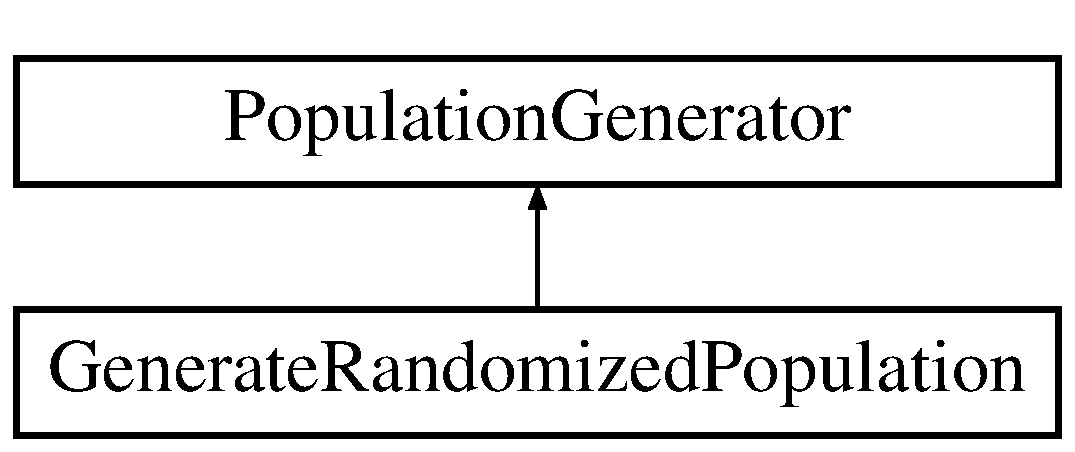
\includegraphics[height=2.000000cm]{class_generate_randomized_population}
\end{center}
\end{figure}
\subsection*{Public Member Functions}
\begin{DoxyCompactItemize}
\item 
\hypertarget{class_generate_randomized_population_aa720b865e885c3a2de5ae3a04569648c}{\hyperlink{class_generate_randomized_population_aa720b865e885c3a2de5ae3a04569648c}{Generate\+Randomized\+Population} ()}\label{class_generate_randomized_population_aa720b865e885c3a2de5ae3a04569648c}

\begin{DoxyCompactList}\small\item\em Constuct function object \hyperlink{class_generate_randomized_population}{Generate\+Randomized\+Population}. \end{DoxyCompactList}\item 
\hypertarget{class_generate_randomized_population_af909ed6bb075e123d4b17f585bddcbf2}{\hyperlink{class_generate_randomized_population_af909ed6bb075e123d4b17f585bddcbf2}{Generate\+Randomized\+Population} (unsigned int seed)}\label{class_generate_randomized_population_af909ed6bb075e123d4b17f585bddcbf2}

\begin{DoxyCompactList}\small\item\em Construct function object \hyperlink{class_generate_randomized_population}{Generate\+Randomized\+Population} with a seed for a predicable population. \end{DoxyCompactList}\item 
\hypertarget{class_generate_randomized_population_ad8183d231b576c56527b350c31cc384d}{std\+::vector$<$ \hyperlink{class_m_m_k_p_solution}{M\+M\+K\+P\+Solution} $>$ \hyperlink{class_generate_randomized_population_ad8183d231b576c56527b350c31cc384d}{operator()} (\hyperlink{class_m_m_k_p_data_set}{M\+M\+K\+P\+Data\+Set} data\+Set, int population\+Size)}\label{class_generate_randomized_population_ad8183d231b576c56527b350c31cc384d}

\begin{DoxyCompactList}\small\item\em Run generator and return a vector of solutions (\hyperlink{class_m_m_k_p_solution}{M\+M\+K\+P\+Solution}). \end{DoxyCompactList}\end{DoxyCompactItemize}


\subsection{Detailed Description}
Generate a feasible, randomized population based on \hyperlink{class_m_m_k_p_data_set}{M\+M\+K\+P\+Data\+Set} for class/item size, feasilbility, profit and cost constraint calculations. 

The documentation for this class was generated from the following files\+:\begin{DoxyCompactItemize}
\item 
M\+M\+K\+P\+Population\+Generators.\+h\item 
M\+M\+K\+P\+Population\+Generators.\+cpp\end{DoxyCompactItemize}

\hypertarget{class_generate_randomized_population_greedy_v1}{\section{Generate\+Randomized\+Population\+Greedy\+V1 Class Reference}
\label{class_generate_randomized_population_greedy_v1}\index{Generate\+Randomized\+Population\+Greedy\+V1@{Generate\+Randomized\+Population\+Greedy\+V1}}
}


A semi random greedy approach.  




{\ttfamily \#include $<$M\+M\+K\+P\+Population\+Generators.\+h$>$}

Inheritance diagram for Generate\+Randomized\+Population\+Greedy\+V1\+:\begin{figure}[H]
\begin{center}
\leavevmode
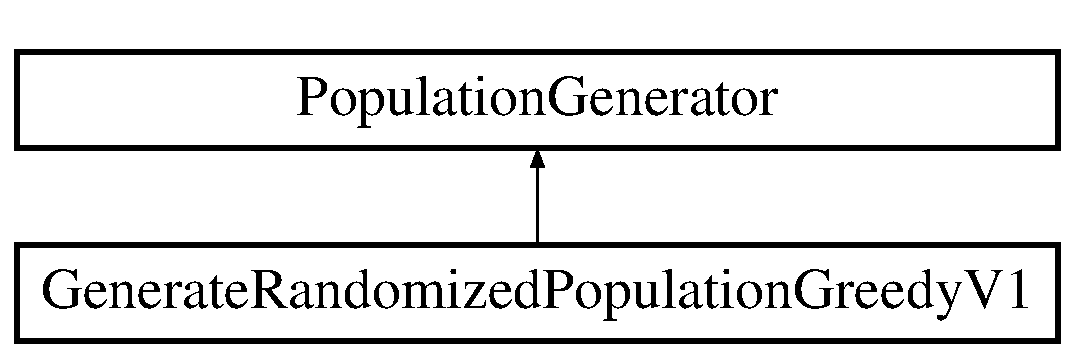
\includegraphics[height=2.000000cm]{class_generate_randomized_population_greedy_v1}
\end{center}
\end{figure}
\subsection*{Public Member Functions}
\begin{DoxyCompactItemize}
\item 
\hypertarget{class_generate_randomized_population_greedy_v1_a8b319a423128a1871a1874fdadbd8573}{\hyperlink{class_generate_randomized_population_greedy_v1_a8b319a423128a1871a1874fdadbd8573}{Generate\+Randomized\+Population\+Greedy\+V1} ()}\label{class_generate_randomized_population_greedy_v1_a8b319a423128a1871a1874fdadbd8573}

\begin{DoxyCompactList}\small\item\em Constuct function object \hyperlink{class_generate_randomized_population_greedy_v1}{Generate\+Randomized\+Population\+Greedy\+V1}. \end{DoxyCompactList}\item 
\hypertarget{class_generate_randomized_population_greedy_v1_a31f380a168ce525bd6f70c54730ab3da}{\hyperlink{class_generate_randomized_population_greedy_v1_a31f380a168ce525bd6f70c54730ab3da}{Generate\+Randomized\+Population\+Greedy\+V1} (unsigned int seed)}\label{class_generate_randomized_population_greedy_v1_a31f380a168ce525bd6f70c54730ab3da}

\begin{DoxyCompactList}\small\item\em Construct function object \hyperlink{class_generate_randomized_population_greedy_v1}{Generate\+Randomized\+Population\+Greedy\+V1} with a seed for a predicable population. \end{DoxyCompactList}\item 
\hypertarget{class_generate_randomized_population_greedy_v1_af39358dbec454c105e04a792df3524d7}{std\+::vector$<$ \hyperlink{class_m_m_k_p_solution}{M\+M\+K\+P\+Solution} $>$ \hyperlink{class_generate_randomized_population_greedy_v1_af39358dbec454c105e04a792df3524d7}{operator()} (\hyperlink{class_m_m_k_p_data_set}{M\+M\+K\+P\+Data\+Set} data\+Set, int population\+Size)}\label{class_generate_randomized_population_greedy_v1_af39358dbec454c105e04a792df3524d7}

\begin{DoxyCompactList}\small\item\em Run generator and return a vector of solutions (\hyperlink{class_m_m_k_p_solution}{M\+M\+K\+P\+Solution}). \end{DoxyCompactList}\end{DoxyCompactItemize}


\subsection{Detailed Description}
A semi random greedy approach. 

This chooses an item to add to a class based on 1 of 5 possible functions for calculating a surrogate profit. 

The documentation for this class was generated from the following files\+:\begin{DoxyCompactItemize}
\item 
M\+M\+K\+P\+Population\+Generators.\+h\item 
M\+M\+K\+P\+Population\+Generators.\+cpp\end{DoxyCompactItemize}

\hypertarget{class_generate_randomized_population_no_dups}{\section{Generate\+Randomized\+Population\+No\+Dups Class Reference}
\label{class_generate_randomized_population_no_dups}\index{Generate\+Randomized\+Population\+No\+Dups@{Generate\+Randomized\+Population\+No\+Dups}}
}


Generate a feasible, randomized population based on \hyperlink{class_m_m_k_p_data_set}{M\+M\+K\+P\+Data\+Set} for class/item size, feasilbility, profit and cost constraint calculations.  




{\ttfamily \#include $<$M\+M\+K\+P\+Population\+Generators.\+h$>$}

Inheritance diagram for Generate\+Randomized\+Population\+No\+Dups\+:\begin{figure}[H]
\begin{center}
\leavevmode
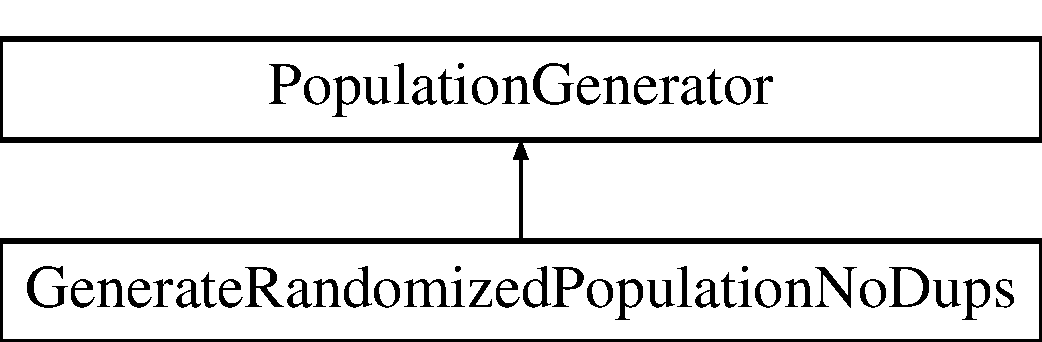
\includegraphics[height=2.000000cm]{class_generate_randomized_population_no_dups}
\end{center}
\end{figure}
\subsection*{Public Member Functions}
\begin{DoxyCompactItemize}
\item 
\hypertarget{class_generate_randomized_population_no_dups_a2daaef37cfadbf99d106720d9516d882}{\hyperlink{class_generate_randomized_population_no_dups_a2daaef37cfadbf99d106720d9516d882}{Generate\+Randomized\+Population\+No\+Dups} ()}\label{class_generate_randomized_population_no_dups_a2daaef37cfadbf99d106720d9516d882}

\begin{DoxyCompactList}\small\item\em Constuct function object \hyperlink{class_generate_randomized_population_no_dups}{Generate\+Randomized\+Population\+No\+Dups}. \end{DoxyCompactList}\item 
\hypertarget{class_generate_randomized_population_no_dups_a3d144613c04fb863924a5311461a985d}{\hyperlink{class_generate_randomized_population_no_dups_a3d144613c04fb863924a5311461a985d}{Generate\+Randomized\+Population\+No\+Dups} (unsigned int seed)}\label{class_generate_randomized_population_no_dups_a3d144613c04fb863924a5311461a985d}

\begin{DoxyCompactList}\small\item\em Construct function object \hyperlink{class_generate_randomized_population_no_dups}{Generate\+Randomized\+Population\+No\+Dups} with a seed for a predicable population. \end{DoxyCompactList}\item 
\hypertarget{class_generate_randomized_population_no_dups_a9fa6bb86573aad1a924cea7908c6c5b6}{std\+::vector$<$ \hyperlink{class_m_m_k_p_solution}{M\+M\+K\+P\+Solution} $>$ \hyperlink{class_generate_randomized_population_no_dups_a9fa6bb86573aad1a924cea7908c6c5b6}{operator()} (\hyperlink{class_m_m_k_p_data_set}{M\+M\+K\+P\+Data\+Set} data\+Set, int population\+Size)}\label{class_generate_randomized_population_no_dups_a9fa6bb86573aad1a924cea7908c6c5b6}

\begin{DoxyCompactList}\small\item\em Run generator and return a vector of solutions (\hyperlink{class_m_m_k_p_solution}{M\+M\+K\+P\+Solution}). \end{DoxyCompactList}\end{DoxyCompactItemize}


\subsection{Detailed Description}
Generate a feasible, randomized population based on \hyperlink{class_m_m_k_p_data_set}{M\+M\+K\+P\+Data\+Set} for class/item size, feasilbility, profit and cost constraint calculations. 

This population does not allow for repeated solutions and does not validate that more solutions exist than the size of population being generated. This would cuase an infinite loop as it is in the best interest of portability that we do not dictate the stopping criterion. 

The documentation for this class was generated from the following files\+:\begin{DoxyCompactItemize}
\item 
M\+M\+K\+P\+Population\+Generators.\+h\item 
M\+M\+K\+P\+Population\+Generators.\+cpp\end{DoxyCompactItemize}

\hypertarget{class_generate_randomized_population_no_dups___infeasible}{\section{Generate\+Randomized\+Population\+No\+Dups\+\_\+\+Infeasible Class Reference}
\label{class_generate_randomized_population_no_dups___infeasible}\index{Generate\+Randomized\+Population\+No\+Dups\+\_\+\+Infeasible@{Generate\+Randomized\+Population\+No\+Dups\+\_\+\+Infeasible}}
}


Generate a feasible, randomized population based on \hyperlink{class_m_m_k_p_data_set}{M\+M\+K\+P\+Data\+Set} for class/item size, feasilbility, profit and cost constraint calculations.  




{\ttfamily \#include $<$M\+M\+K\+P\+Population\+Generators.\+h$>$}

Inheritance diagram for Generate\+Randomized\+Population\+No\+Dups\+\_\+\+Infeasible\+:\begin{figure}[H]
\begin{center}
\leavevmode
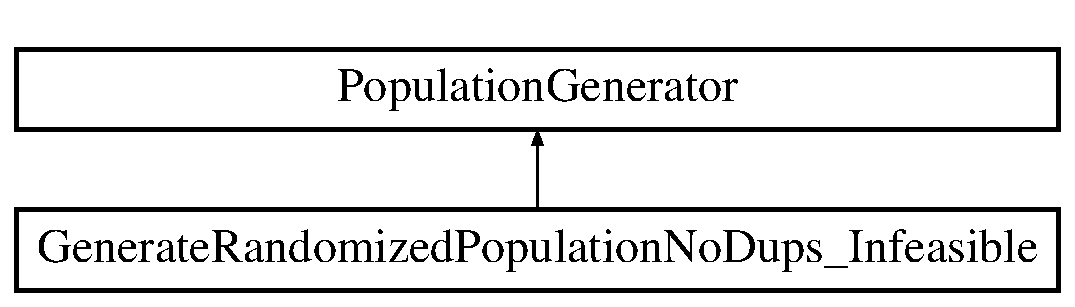
\includegraphics[height=2.000000cm]{class_generate_randomized_population_no_dups___infeasible}
\end{center}
\end{figure}
\subsection*{Public Member Functions}
\begin{DoxyCompactItemize}
\item 
\hypertarget{class_generate_randomized_population_no_dups___infeasible_a059a40654b381b09fc833bcbaee00499}{\hyperlink{class_generate_randomized_population_no_dups___infeasible_a059a40654b381b09fc833bcbaee00499}{Generate\+Randomized\+Population\+No\+Dups\+\_\+\+Infeasible} ()}\label{class_generate_randomized_population_no_dups___infeasible_a059a40654b381b09fc833bcbaee00499}

\begin{DoxyCompactList}\small\item\em Constuct function object \hyperlink{class_generate_randomized_population_no_dups___infeasible}{Generate\+Randomized\+Population\+No\+Dups\+\_\+\+Infeasible}. \end{DoxyCompactList}\item 
\hypertarget{class_generate_randomized_population_no_dups___infeasible_a7a679a8fec57e8400511c874777502b4}{\hyperlink{class_generate_randomized_population_no_dups___infeasible_a7a679a8fec57e8400511c874777502b4}{Generate\+Randomized\+Population\+No\+Dups\+\_\+\+Infeasible} (unsigned int seed)}\label{class_generate_randomized_population_no_dups___infeasible_a7a679a8fec57e8400511c874777502b4}

\begin{DoxyCompactList}\small\item\em Construct function object \hyperlink{class_generate_randomized_population_no_dups___infeasible}{Generate\+Randomized\+Population\+No\+Dups\+\_\+\+Infeasible} with a seed for a predicable population. \end{DoxyCompactList}\item 
\hypertarget{class_generate_randomized_population_no_dups___infeasible_a18dc0daab30c2924f0f1596bd6e4ef48}{std\+::vector$<$ \hyperlink{class_m_m_k_p_solution}{M\+M\+K\+P\+Solution} $>$ \hyperlink{class_generate_randomized_population_no_dups___infeasible_a18dc0daab30c2924f0f1596bd6e4ef48}{operator()} (\hyperlink{class_m_m_k_p_data_set}{M\+M\+K\+P\+Data\+Set} data\+Set, int population\+Size)}\label{class_generate_randomized_population_no_dups___infeasible_a18dc0daab30c2924f0f1596bd6e4ef48}

\begin{DoxyCompactList}\small\item\em Run generator and return a vector of solutions (\hyperlink{class_m_m_k_p_solution}{M\+M\+K\+P\+Solution}). \end{DoxyCompactList}\end{DoxyCompactItemize}


\subsection{Detailed Description}
Generate a feasible, randomized population based on \hyperlink{class_m_m_k_p_data_set}{M\+M\+K\+P\+Data\+Set} for class/item size, feasilbility, profit and cost constraint calculations. 

This population does not allow for repeated solutions and does not validate that more solutions exist than the size of population being generated. This would cuase an infinite loop as it is in the best interest of portability that we do not dictate the stopping criterion. This population may also violate multiple dimension feasibility. 

The documentation for this class was generated from the following files\+:\begin{DoxyCompactItemize}
\item 
M\+M\+K\+P\+Population\+Generators.\+h\item 
M\+M\+K\+P\+Population\+Generators.\+cpp\end{DoxyCompactItemize}

\hypertarget{class_hiremath_hill___read}{\section{Hiremath\+Hill\+\_\+\+Read Class Reference}
\label{class_hiremath_hill___read}\index{Hiremath\+Hill\+\_\+\+Read@{Hiremath\+Hill\+\_\+\+Read}}
}


Hiremath\+Hill Function Object reads from Hiremath\+Hill problem sets and converts to common format \hyperlink{class_m_m_k_p_data_set}{M\+M\+K\+P\+Data\+Set}.  




{\ttfamily \#include $<$M\+M\+K\+P\+Data\+Set.\+h$>$}

\subsection*{Public Member Functions}
\begin{DoxyCompactItemize}
\item 
\hyperlink{class_m_m_k_p_data_set}{M\+M\+K\+P\+Data\+Set} \hyperlink{class_hiremath_hill___read_a65f20d16d8b49e5e6b5d217e7c2dcb51}{operator()} (std\+::ifstream \&file, int problem\+To\+Run)
\begin{DoxyCompactList}\small\item\em Convert input file to \hyperlink{class_m_m_k_p_data_set}{M\+M\+K\+P\+Data\+Set}. \end{DoxyCompactList}\end{DoxyCompactItemize}


\subsection{Detailed Description}
Hiremath\+Hill Function Object reads from Hiremath\+Hill problem sets and converts to common format \hyperlink{class_m_m_k_p_data_set}{M\+M\+K\+P\+Data\+Set}. 

\subsection{Member Function Documentation}
\hypertarget{class_hiremath_hill___read_a65f20d16d8b49e5e6b5d217e7c2dcb51}{\index{Hiremath\+Hill\+\_\+\+Read@{Hiremath\+Hill\+\_\+\+Read}!operator()@{operator()}}
\index{operator()@{operator()}!Hiremath\+Hill\+\_\+\+Read@{Hiremath\+Hill\+\_\+\+Read}}
\subsubsection[{operator()}]{\setlength{\rightskip}{0pt plus 5cm}{\bf M\+M\+K\+P\+Data\+Set} Hiremath\+Hill\+\_\+\+Read\+::operator() (
\begin{DoxyParamCaption}
\item[{std\+::ifstream \&}]{file, }
\item[{int}]{problem\+To\+Run}
\end{DoxyParamCaption}
)}}\label{class_hiremath_hill___read_a65f20d16d8b49e5e6b5d217e7c2dcb51}


Convert input file to \hyperlink{class_m_m_k_p_data_set}{M\+M\+K\+P\+Data\+Set}. 

Since each file in the Hiremath/\+Hill problem set has multuple problems, a problem to run may be specified (starting at index 1). 

The documentation for this class was generated from the following files\+:\begin{DoxyCompactItemize}
\item 
M\+M\+K\+P\+Data\+Set.\+h\item 
M\+M\+K\+P\+Data\+Set.\+cpp\end{DoxyCompactItemize}

\hypertarget{class_item_data}{\section{Item\+Data Class Reference}
\label{class_item_data}\index{Item\+Data@{Item\+Data}}
}


Item in M\+M\+K\+P, which consists of a profit and cost for each constraint.  




{\ttfamily \#include $<$M\+M\+K\+P\+Data\+Set.\+h$>$}

\subsection*{Public Member Functions}
\begin{DoxyCompactItemize}
\item 
\hypertarget{class_item_data_a3a1b6240b016a82fa65b450f98a35f6c}{\hyperlink{class_item_data_a3a1b6240b016a82fa65b450f98a35f6c}{Item\+Data} ()}\label{class_item_data_a3a1b6240b016a82fa65b450f98a35f6c}

\begin{DoxyCompactList}\small\item\em Construct empty \hyperlink{class_item_data}{Item\+Data}. \end{DoxyCompactList}\item 
\hyperlink{class_item_data_a724e9978670f3dc3160e0e5128b7001e}{Item\+Data} (float profit, std\+::vector$<$ float $>$ costs, std\+::vector$<$ float $>$ problem\+Resources)
\begin{DoxyCompactList}\small\item\em Construct \hyperlink{class_item_data}{Item\+Data}. \end{DoxyCompactList}\item 
\hypertarget{class_item_data_af44bf5f67511a8249f7edc7f9e501fb5}{float \hyperlink{class_item_data_af44bf5f67511a8249f7edc7f9e501fb5}{get\+Profit} () const }\label{class_item_data_af44bf5f67511a8249f7edc7f9e501fb5}

\begin{DoxyCompactList}\small\item\em Return profit of \hyperlink{class_item_data}{Item\+Data}. \end{DoxyCompactList}\item 
\hypertarget{class_item_data_a9341a1a66ac5933ef7dcf217074a05c2}{std\+::vector$<$ float $>$ \hyperlink{class_item_data_a9341a1a66ac5933ef7dcf217074a05c2}{get\+Costs} () const }\label{class_item_data_a9341a1a66ac5933ef7dcf217074a05c2}

\begin{DoxyCompactList}\small\item\em Return costs of constraints for \hyperlink{class_item_data}{Item\+Data}. \end{DoxyCompactList}\item 
float \hyperlink{class_item_data_a8746e271ee49c40c1f5def099478e840}{get\+Cost} (int index) const 
\begin{DoxyCompactList}\small\item\em Return cost of a constraint for \hyperlink{class_item_data}{Item\+Data}. \end{DoxyCompactList}\item 
\hypertarget{class_item_data_aa75225399919410086ee0c7f766c315d}{int \hyperlink{class_item_data_aa75225399919410086ee0c7f766c315d}{get\+Number\+Of\+Costs} () const }\label{class_item_data_aa75225399919410086ee0c7f766c315d}

\begin{DoxyCompactList}\small\item\em Return the number of constraints for \hyperlink{class_item_data}{Item\+Data}. \end{DoxyCompactList}\item 
\hypertarget{class_item_data_ae5e1ad22dd903359d35798e6cdcb9b2b}{float \hyperlink{class_item_data_ae5e1ad22dd903359d35798e6cdcb9b2b}{get\+Profit\+Constraint\+Use\+Percent} () const }\label{class_item_data_ae5e1ad22dd903359d35798e6cdcb9b2b}

\begin{DoxyCompactList}\small\item\em Return v/\mbox{[}Er\%/n\mbox{]} for a \hyperlink{class_item_data}{Item\+Data}. \end{DoxyCompactList}\item 
\hypertarget{class_item_data_aa2511a10c0c9e51ad6bcea213f1e3e86}{float \hyperlink{class_item_data_aa2511a10c0c9e51ad6bcea213f1e3e86}{get\+Profit\+Constraint\+Use\+Percent} (std\+::vector$<$ int $>$ indices) const }\label{class_item_data_aa2511a10c0c9e51ad6bcea213f1e3e86}

\begin{DoxyCompactList}\small\item\em Return v/\mbox{[}Er\%/n\mbox{]} for a \hyperlink{class_item_data}{Item\+Data}, using only certain indices. \end{DoxyCompactList}\item 
\hypertarget{class_item_data_afca53a09768f49cc97726da9551d8631}{float \hyperlink{class_item_data_afca53a09768f49cc97726da9551d8631}{get\+Constraint\+Use\+Percent} () const }\label{class_item_data_afca53a09768f49cc97726da9551d8631}

\begin{DoxyCompactList}\small\item\em Return Er\%/n for \hyperlink{class_item_data}{Item\+Data}. \end{DoxyCompactList}\item 
\hypertarget{class_item_data_a2735e611eb49cd7b55ee56e3b834f0d4}{float {\bfseries get\+Constraint\+Use\+Percent} (int index)}\label{class_item_data_a2735e611eb49cd7b55ee56e3b834f0d4}

\item 
\hypertarget{class_item_data_a3b0a42c28b6b4db4a2bf31d2c370cd0c}{float {\bfseries get\+Profit\+Constraint\+Use\+Percent} (int index)}\label{class_item_data_a3b0a42c28b6b4db4a2bf31d2c370cd0c}

\item 
\hypertarget{class_item_data_af526fb020485fce4bd68bbf003e18f37}{float {\bfseries get\+Constraint\+Use\+Percent} (std\+::vector$<$ int $>$ indices)}\label{class_item_data_af526fb020485fce4bd68bbf003e18f37}

\item 
\hypertarget{class_item_data_a79caed963f73c2ca4aefaae49c8ea1b1}{void \hyperlink{class_item_data_a79caed963f73c2ca4aefaae49c8ea1b1}{set\+Profit} (const float profit)}\label{class_item_data_a79caed963f73c2ca4aefaae49c8ea1b1}

\begin{DoxyCompactList}\small\item\em Set profit for an \hyperlink{class_item_data}{Item\+Data}. \end{DoxyCompactList}\item 
void \hyperlink{class_item_data_a6bc1758713f145a8821d57c40547c2cb}{set\+Costs} (const std\+::vector$<$ float $>$ costs)
\begin{DoxyCompactList}\small\item\em Set Costs of all constraints for an \hyperlink{class_item_data}{Item\+Data}. \end{DoxyCompactList}\item 
void \hyperlink{class_item_data_a138d46bf17af403471f4bf46a8e44d50}{set\+Analytics} (const std\+::vector$<$ float $>$ problem\+Resources)
\begin{DoxyCompactList}\small\item\em Set all \hyperlink{class_item_data}{Item\+Data} analytic measures. \end{DoxyCompactList}\end{DoxyCompactItemize}


\subsection{Detailed Description}
Item in M\+M\+K\+P, which consists of a profit and cost for each constraint. 

\subsection{Constructor \& Destructor Documentation}
\hypertarget{class_item_data_a724e9978670f3dc3160e0e5128b7001e}{\index{Item\+Data@{Item\+Data}!Item\+Data@{Item\+Data}}
\index{Item\+Data@{Item\+Data}!Item\+Data@{Item\+Data}}
\subsubsection[{Item\+Data}]{\setlength{\rightskip}{0pt plus 5cm}Item\+Data\+::\+Item\+Data (
\begin{DoxyParamCaption}
\item[{float}]{profit, }
\item[{std\+::vector$<$ float $>$}]{costs, }
\item[{std\+::vector$<$ float $>$}]{problem\+Resources}
\end{DoxyParamCaption}
)}}\label{class_item_data_a724e9978670f3dc3160e0e5128b7001e}


Construct \hyperlink{class_item_data}{Item\+Data}. 

Param\+: Problem\+Resources used in analytic functions, can also use set\+Analytics instead of this constructor. 

\subsection{Member Function Documentation}
\hypertarget{class_item_data_a8746e271ee49c40c1f5def099478e840}{\index{Item\+Data@{Item\+Data}!get\+Cost@{get\+Cost}}
\index{get\+Cost@{get\+Cost}!Item\+Data@{Item\+Data}}
\subsubsection[{get\+Cost}]{\setlength{\rightskip}{0pt plus 5cm}float Item\+Data\+::get\+Cost (
\begin{DoxyParamCaption}
\item[{int}]{index}
\end{DoxyParamCaption}
) const}}\label{class_item_data_a8746e271ee49c40c1f5def099478e840}


Return cost of a constraint for \hyperlink{class_item_data}{Item\+Data}. 

Parameter index corresponds to the cost of one constraint, starting a index 0. \hypertarget{class_item_data_a138d46bf17af403471f4bf46a8e44d50}{\index{Item\+Data@{Item\+Data}!set\+Analytics@{set\+Analytics}}
\index{set\+Analytics@{set\+Analytics}!Item\+Data@{Item\+Data}}
\subsubsection[{set\+Analytics}]{\setlength{\rightskip}{0pt plus 5cm}void Item\+Data\+::set\+Analytics (
\begin{DoxyParamCaption}
\item[{const std\+::vector$<$ float $>$}]{problem\+Resources}
\end{DoxyParamCaption}
)}}\label{class_item_data_a138d46bf17af403471f4bf46a8e44d50}


Set all \hyperlink{class_item_data}{Item\+Data} analytic measures. 

This includes Er\%/n and v/\mbox{[}Er\%/n\mbox{]} values. \hypertarget{class_item_data_a6bc1758713f145a8821d57c40547c2cb}{\index{Item\+Data@{Item\+Data}!set\+Costs@{set\+Costs}}
\index{set\+Costs@{set\+Costs}!Item\+Data@{Item\+Data}}
\subsubsection[{set\+Costs}]{\setlength{\rightskip}{0pt plus 5cm}void Item\+Data\+::set\+Costs (
\begin{DoxyParamCaption}
\item[{const std\+::vector$<$ float $>$}]{costs}
\end{DoxyParamCaption}
)}}\label{class_item_data_a6bc1758713f145a8821d57c40547c2cb}


Set Costs of all constraints for an \hyperlink{class_item_data}{Item\+Data}. 

This will override all costs previously set. 

The documentation for this class was generated from the following files\+:\begin{DoxyCompactItemize}
\item 
M\+M\+K\+P\+Data\+Set.\+h\item 
M\+M\+K\+P\+Data\+Set.\+cpp\end{DoxyCompactItemize}

\hypertarget{class_m_m_k_p___t_l_b_o}{\section{M\+M\+K\+P\+\_\+\+T\+L\+B\+O Class Reference}
\label{class_m_m_k_p___t_l_b_o}\index{M\+M\+K\+P\+\_\+\+T\+L\+B\+O@{M\+M\+K\+P\+\_\+\+T\+L\+B\+O}}
}


Teaching-\/learning-\/based optimization algrithm for the multiple-\/choice, multiple-\/dimensional knapsack problem.  




{\ttfamily \#include $<$M\+M\+K\+P\+\_\+\+T\+L\+B\+O.\+h$>$}

\subsection*{Public Member Functions}
\begin{DoxyCompactItemize}
\item 
\hyperlink{class_m_m_k_p___t_l_b_o_a889c073268b283872a9601616bfcf6b0}{M\+M\+K\+P\+\_\+\+T\+L\+B\+O} (\hyperlink{class_m_m_k_p_data_set}{M\+M\+K\+P\+Data\+Set} data\+Set, \hyperlink{struct_t_l_b_o__parameters}{T\+L\+B\+O\+\_\+parameters} parameters)
\begin{DoxyCompactList}\small\item\em Construct \hyperlink{class_m_m_k_p___t_l_b_o}{M\+M\+K\+P\+\_\+\+T\+L\+B\+O} object. \end{DoxyCompactList}\item 
\hypertarget{class_m_m_k_p___t_l_b_o_a095c049b8f168b34f2287a9cdbe5cd71}{\hyperlink{class_m_m_k_p_solution}{M\+M\+K\+P\+Solution} \hyperlink{class_m_m_k_p___t_l_b_o_a095c049b8f168b34f2287a9cdbe5cd71}{operator()} (std\+::vector$<$ \hyperlink{class_m_m_k_p_solution}{M\+M\+K\+P\+Solution} $>$ initial\+Population)}\label{class_m_m_k_p___t_l_b_o_a095c049b8f168b34f2287a9cdbe5cd71}

\begin{DoxyCompactList}\small\item\em Run tlbo algorithm and return the result, which is the 'teaching' solution after a stopping criterion is met. \end{DoxyCompactList}\item 
\hypertarget{class_m_m_k_p___t_l_b_o_aaf6f0fddc9df079743b0bd2ca8414713}{float \hyperlink{class_m_m_k_p___t_l_b_o_aaf6f0fddc9df079743b0bd2ca8414713}{get\+Acceptance\+Rate} ()}\label{class_m_m_k_p___t_l_b_o_aaf6f0fddc9df079743b0bd2ca8414713}

\begin{DoxyCompactList}\small\item\em Return percent of total mutations done to all solutions from last run of tlbo algorithm that were accepted as feasible and had an increased profit. \end{DoxyCompactList}\item 
\hypertarget{class_m_m_k_p___t_l_b_o_a5fc9b7ea967e88f473063dc91fe45b5c}{float \hyperlink{class_m_m_k_p___t_l_b_o_a5fc9b7ea967e88f473063dc91fe45b5c}{get\+Feasbility\+Rate} ()}\label{class_m_m_k_p___t_l_b_o_a5fc9b7ea967e88f473063dc91fe45b5c}

\begin{DoxyCompactList}\small\item\em Return percent of solutions able to be made feasible after being in an infeasible state from the teaching or learning stage of T\+L\+B\+O. \end{DoxyCompactList}\item 
\hypertarget{class_m_m_k_p___t_l_b_o_af376e7f0515c68e0306028bc724ccb19}{int \hyperlink{class_m_m_k_p___t_l_b_o_af376e7f0515c68e0306028bc724ccb19}{get\+Number\+Of\+Unique\+Solutions} ()}\label{class_m_m_k_p___t_l_b_o_af376e7f0515c68e0306028bc724ccb19}

\begin{DoxyCompactList}\small\item\em Return number of unique solutions from last T\+L\+B\+O run . \end{DoxyCompactList}\item 
void \hyperlink{class_m_m_k_p___t_l_b_o_aec2c0d19229e361d745740bacf10b679}{add\+To\+Unique\+Solution\+Set} (\hyperlink{class_m_m_k_p_solution}{M\+M\+K\+P\+Solution} sol)
\begin{DoxyCompactList}\small\item\em Add to unqiue solution set. \end{DoxyCompactList}\item 
void \hyperlink{class_m_m_k_p___t_l_b_o_a40f0e094b6dff74ff91d0e0d7c4a27e9}{quick\+Sort} (std\+::vector$<$ \hyperlink{class_m_m_k_p_solution}{M\+M\+K\+P\+Solution} $>$ \&input, int p, int r)
\begin{DoxyCompactList}\small\item\em Sort a population of \hyperlink{class_m_m_k_p_solution}{M\+M\+K\+P\+Solution}'s using quicksort. \end{DoxyCompactList}\item 
\hypertarget{class_m_m_k_p___t_l_b_o_a53c91633b431434f6179202486642214}{int \hyperlink{class_m_m_k_p___t_l_b_o_a53c91633b431434f6179202486642214}{partition} (std\+::vector$<$ \hyperlink{class_m_m_k_p_solution}{M\+M\+K\+P\+Solution} $>$ \&input, int p, int r)}\label{class_m_m_k_p___t_l_b_o_a53c91633b431434f6179202486642214}

\begin{DoxyCompactList}\small\item\em Quicksort helper funtion. \end{DoxyCompactList}\item 
\hypertarget{class_m_m_k_p___t_l_b_o_accea97f95a12f373c6a0907804de0db8}{\hyperlink{class_m_m_k_p_solution}{M\+M\+K\+P\+Solution} \hyperlink{class_m_m_k_p___t_l_b_o_accea97f95a12f373c6a0907804de0db8}{run} (std\+::vector$<$ \hyperlink{class_m_m_k_p_solution}{M\+M\+K\+P\+Solution} $>$ initial\+Population)}\label{class_m_m_k_p___t_l_b_o_accea97f95a12f373c6a0907804de0db8}

\begin{DoxyCompactList}\small\item\em Run tlbo algorithm and return the result, which is the 'teaching' solution after a stopping criterion is met. \end{DoxyCompactList}\item 
void \hyperlink{class_m_m_k_p___t_l_b_o_ab18aa71ce62a00663cedb6d7d8db6f38}{teaching\+Phase} (std\+::vector$<$ \hyperlink{class_m_m_k_p_solution}{M\+M\+K\+P\+Solution} $>$ \&population)
\begin{DoxyCompactList}\small\item\em T\+L\+B\+O teaching phase. \end{DoxyCompactList}\item 
void \hyperlink{class_m_m_k_p___t_l_b_o_a0d3fe3e2570a79a3bd2f29aef3977d7e}{teaching\+Phase\+\_\+\+Multi\+Teacher} (std\+::vector$<$ \hyperlink{class_m_m_k_p_solution}{M\+M\+K\+P\+Solution} $>$ \&population, int class\+Size)
\begin{DoxyCompactList}\small\item\em i-\/\+T\+L\+B\+O teaching phase. \end{DoxyCompactList}\item 
void \hyperlink{class_m_m_k_p___t_l_b_o_a6377147784c758b4f8e782b37f86be73}{teaching\+Phase\+\_\+\+Orthognal} (std\+::vector$<$ \hyperlink{class_m_m_k_p_solution}{M\+M\+K\+P\+Solution} $>$ \&population, int iteration)
\begin{DoxyCompactList}\small\item\em O-\/\+T\+L\+B\+O teaching phase. \end{DoxyCompactList}\item 
void \hyperlink{class_m_m_k_p___t_l_b_o_ae230bdd3c27355b3b89c23ba3de2cb29}{learning\+Phase} (std\+::vector$<$ \hyperlink{class_m_m_k_p_solution}{M\+M\+K\+P\+Solution} $>$ \&population)
\begin{DoxyCompactList}\small\item\em T\+L\+B\+O learning phase. \end{DoxyCompactList}\item 
void \hyperlink{class_m_m_k_p___t_l_b_o_ad79c49be3f52a25879df07ad70af65d8}{learning\+Phase\+\_\+\+Orthognal} (std\+::vector$<$ \hyperlink{class_m_m_k_p_solution}{M\+M\+K\+P\+Solution} $>$ \&population, int iteration)
\begin{DoxyCompactList}\small\item\em O-\/\+T\+L\+B\+O learning phase. \end{DoxyCompactList}\item 
\hypertarget{class_m_m_k_p___t_l_b_o_a2edb2de3b8f71f7df34812be858e752a}{bool \hyperlink{class_m_m_k_p___t_l_b_o_a2edb2de3b8f71f7df34812be858e752a}{make\+Feasible} (\hyperlink{class_m_m_k_p_solution}{M\+M\+K\+P\+Solution} \&sol)}\label{class_m_m_k_p___t_l_b_o_a2edb2de3b8f71f7df34812be858e752a}

\begin{DoxyCompactList}\small\item\em Wrapper function for feasibility routines. \end{DoxyCompactList}\item 
bool \hyperlink{class_m_m_k_p___t_l_b_o_a663310e7f122715a3c90a0f9839eb69f}{make\+Feasible} (\hyperlink{class_m_m_k_p_solution}{M\+M\+K\+P\+Solution} \&sol, int mc\+Feas, int md\+Feas)
\begin{DoxyCompactList}\small\item\em Wrapper function for feasiblity routines. \end{DoxyCompactList}\item 
bool \hyperlink{class_m_m_k_p___t_l_b_o_ac49eccf57219c4973cdae02b6e7a6e08}{make\+Multi\+Choice\+Feas\+Fixed\+Surrogate} (\hyperlink{class_m_m_k_p_solution}{M\+M\+K\+P\+Solution} \&sol)
\begin{DoxyCompactList}\small\item\em Make multi-\/choice feasible based a surrogate constraint created using all costs in an item. \end{DoxyCompactList}\item 
bool \hyperlink{class_m_m_k_p___t_l_b_o_a49ab01792695f1282e28eacf157c0dca}{make\+Multi\+Choice\+Feas\+Fixed\+\_\+\+Rand\+\_\+\+Surrogate} (\hyperlink{class_m_m_k_p_solution}{M\+M\+K\+P\+Solution} \&sol)
\begin{DoxyCompactList}\small\item\em Make multi-\/choice feasible based a surrogate constraint created using all costs in an item. \end{DoxyCompactList}\item 
bool \hyperlink{class_m_m_k_p___t_l_b_o_a6e466ab9f14bab8e1107c15867628e11}{make\+Multi\+Choice\+Feas\+Max\+Profit} (\hyperlink{class_m_m_k_p_solution}{M\+M\+K\+P\+Solution} \&sol)
\begin{DoxyCompactList}\small\item\em Make multi-\/choice feasible based on profit alone. \end{DoxyCompactList}\item 
bool \hyperlink{class_m_m_k_p___t_l_b_o_aa3c59da0a24ef64da308b5801e989e44}{make\+Multi\+Dim\+Feas\+Fixed\+Surrogate} (\hyperlink{class_m_m_k_p_solution}{M\+M\+K\+P\+Solution} \&sol)
\begin{DoxyCompactList}\small\item\em Make multi-\/dim feasible based a surrogate constraint created using all costs in an item. \end{DoxyCompactList}\item 
bool \hyperlink{class_m_m_k_p___t_l_b_o_a91e13c12bc7dd0101d9da358e52eb56c}{make\+Multi\+Dim\+Feas\+Variable\+Surrogate} (\hyperlink{class_m_m_k_p_solution}{M\+M\+K\+P\+Solution} \&sol)
\begin{DoxyCompactList}\small\item\em Make multi-\/dim feasible based a surrogate constraint created using variable number of item's costs's (depending on which violate the problem's resources. \end{DoxyCompactList}\item 
bool \hyperlink{class_m_m_k_p___t_l_b_o_a7b73048fc15101a576b64f3f03520691}{make\+Multi\+Dim\+Feas\+Var\+Min\+Surrogate} (\hyperlink{class_m_m_k_p_solution}{M\+M\+K\+P\+Solution} \&sol)
\begin{DoxyCompactList}\small\item\em Make multi-\/dim feasible based a surrogate constraint created using variable number of item's costs's (depending on which violate the problem's resources. \end{DoxyCompactList}\item 
bool \hyperlink{class_m_m_k_p___t_l_b_o_aea788f9954bf5c56edd8643554d70177}{make\+Multi\+Dim\+Feas\+Var\+Maximize\+Profit} (\hyperlink{class_m_m_k_p_solution}{M\+M\+K\+P\+Solution} \&sol)
\begin{DoxyCompactList}\small\item\em Make multi-\/dim feasible based on maximizing profit. \end{DoxyCompactList}\end{DoxyCompactItemize}


\subsection{Detailed Description}
Teaching-\/learning-\/based optimization algrithm for the multiple-\/choice, multiple-\/dimensional knapsack problem. 

\subsection{Constructor \& Destructor Documentation}
\hypertarget{class_m_m_k_p___t_l_b_o_a889c073268b283872a9601616bfcf6b0}{\index{M\+M\+K\+P\+\_\+\+T\+L\+B\+O@{M\+M\+K\+P\+\_\+\+T\+L\+B\+O}!M\+M\+K\+P\+\_\+\+T\+L\+B\+O@{M\+M\+K\+P\+\_\+\+T\+L\+B\+O}}
\index{M\+M\+K\+P\+\_\+\+T\+L\+B\+O@{M\+M\+K\+P\+\_\+\+T\+L\+B\+O}!M\+M\+K\+P\+\_\+\+T\+L\+B\+O@{M\+M\+K\+P\+\_\+\+T\+L\+B\+O}}
\subsubsection[{M\+M\+K\+P\+\_\+\+T\+L\+B\+O}]{\setlength{\rightskip}{0pt plus 5cm}M\+M\+K\+P\+\_\+\+T\+L\+B\+O\+::\+M\+M\+K\+P\+\_\+\+T\+L\+B\+O (
\begin{DoxyParamCaption}
\item[{{\bf M\+M\+K\+P\+Data\+Set}}]{data\+Set, }
\item[{{\bf T\+L\+B\+O\+\_\+parameters}}]{parameters}
\end{DoxyParamCaption}
)}}\label{class_m_m_k_p___t_l_b_o_a889c073268b283872a9601616bfcf6b0}


Construct \hyperlink{class_m_m_k_p___t_l_b_o}{M\+M\+K\+P\+\_\+\+T\+L\+B\+O} object. 

Param\+: parameters can customize the tlbo algorithm according to struct \hyperlink{struct_t_l_b_o__parameters}{T\+L\+B\+O\+\_\+parameters}. 

\subsection{Member Function Documentation}
\hypertarget{class_m_m_k_p___t_l_b_o_aec2c0d19229e361d745740bacf10b679}{\index{M\+M\+K\+P\+\_\+\+T\+L\+B\+O@{M\+M\+K\+P\+\_\+\+T\+L\+B\+O}!add\+To\+Unique\+Solution\+Set@{add\+To\+Unique\+Solution\+Set}}
\index{add\+To\+Unique\+Solution\+Set@{add\+To\+Unique\+Solution\+Set}!M\+M\+K\+P\+\_\+\+T\+L\+B\+O@{M\+M\+K\+P\+\_\+\+T\+L\+B\+O}}
\subsubsection[{add\+To\+Unique\+Solution\+Set}]{\setlength{\rightskip}{0pt plus 5cm}void M\+M\+K\+P\+\_\+\+T\+L\+B\+O\+::add\+To\+Unique\+Solution\+Set (
\begin{DoxyParamCaption}
\item[{{\bf M\+M\+K\+P\+Solution}}]{sol}
\end{DoxyParamCaption}
)}}\label{class_m_m_k_p___t_l_b_o_aec2c0d19229e361d745740bacf10b679}


Add to unqiue solution set. 

If Solution exists this function does nothing, and if not it will be added to unique solutions list. \hypertarget{class_m_m_k_p___t_l_b_o_ae230bdd3c27355b3b89c23ba3de2cb29}{\index{M\+M\+K\+P\+\_\+\+T\+L\+B\+O@{M\+M\+K\+P\+\_\+\+T\+L\+B\+O}!learning\+Phase@{learning\+Phase}}
\index{learning\+Phase@{learning\+Phase}!M\+M\+K\+P\+\_\+\+T\+L\+B\+O@{M\+M\+K\+P\+\_\+\+T\+L\+B\+O}}
\subsubsection[{learning\+Phase}]{\setlength{\rightskip}{0pt plus 5cm}void M\+M\+K\+P\+\_\+\+T\+L\+B\+O\+::learning\+Phase (
\begin{DoxyParamCaption}
\item[{std\+::vector$<$ {\bf M\+M\+K\+P\+Solution} $>$ \&}]{population}
\end{DoxyParamCaption}
)}}\label{class_m_m_k_p___t_l_b_o_ae230bdd3c27355b3b89c23ba3de2cb29}


T\+L\+B\+O learning phase. 

See Vasko et al. paper for more. \hypertarget{class_m_m_k_p___t_l_b_o_ad79c49be3f52a25879df07ad70af65d8}{\index{M\+M\+K\+P\+\_\+\+T\+L\+B\+O@{M\+M\+K\+P\+\_\+\+T\+L\+B\+O}!learning\+Phase\+\_\+\+Orthognal@{learning\+Phase\+\_\+\+Orthognal}}
\index{learning\+Phase\+\_\+\+Orthognal@{learning\+Phase\+\_\+\+Orthognal}!M\+M\+K\+P\+\_\+\+T\+L\+B\+O@{M\+M\+K\+P\+\_\+\+T\+L\+B\+O}}
\subsubsection[{learning\+Phase\+\_\+\+Orthognal}]{\setlength{\rightskip}{0pt plus 5cm}void M\+M\+K\+P\+\_\+\+T\+L\+B\+O\+::learning\+Phase\+\_\+\+Orthognal (
\begin{DoxyParamCaption}
\item[{std\+::vector$<$ {\bf M\+M\+K\+P\+Solution} $>$ \&}]{population, }
\item[{int}]{iteration}
\end{DoxyParamCaption}
)}}\label{class_m_m_k_p___t_l_b_o_ad79c49be3f52a25879df07ad70af65d8}


O-\/\+T\+L\+B\+O learning phase. 

The learning phase has been modified... \hypertarget{class_m_m_k_p___t_l_b_o_a663310e7f122715a3c90a0f9839eb69f}{\index{M\+M\+K\+P\+\_\+\+T\+L\+B\+O@{M\+M\+K\+P\+\_\+\+T\+L\+B\+O}!make\+Feasible@{make\+Feasible}}
\index{make\+Feasible@{make\+Feasible}!M\+M\+K\+P\+\_\+\+T\+L\+B\+O@{M\+M\+K\+P\+\_\+\+T\+L\+B\+O}}
\subsubsection[{make\+Feasible}]{\setlength{\rightskip}{0pt plus 5cm}bool M\+M\+K\+P\+\_\+\+T\+L\+B\+O\+::make\+Feasible (
\begin{DoxyParamCaption}
\item[{{\bf M\+M\+K\+P\+Solution} \&}]{sol, }
\item[{int}]{mc\+Feas, }
\item[{int}]{md\+Feas}
\end{DoxyParamCaption}
)}}\label{class_m_m_k_p___t_l_b_o_a663310e7f122715a3c90a0f9839eb69f}


Wrapper function for feasiblity routines. 

Uses function parameters instead of Parameters struct to dictate which feasibilty algorithm to apply. \hypertarget{class_m_m_k_p___t_l_b_o_a49ab01792695f1282e28eacf157c0dca}{\index{M\+M\+K\+P\+\_\+\+T\+L\+B\+O@{M\+M\+K\+P\+\_\+\+T\+L\+B\+O}!make\+Multi\+Choice\+Feas\+Fixed\+\_\+\+Rand\+\_\+\+Surrogate@{make\+Multi\+Choice\+Feas\+Fixed\+\_\+\+Rand\+\_\+\+Surrogate}}
\index{make\+Multi\+Choice\+Feas\+Fixed\+\_\+\+Rand\+\_\+\+Surrogate@{make\+Multi\+Choice\+Feas\+Fixed\+\_\+\+Rand\+\_\+\+Surrogate}!M\+M\+K\+P\+\_\+\+T\+L\+B\+O@{M\+M\+K\+P\+\_\+\+T\+L\+B\+O}}
\subsubsection[{make\+Multi\+Choice\+Feas\+Fixed\+\_\+\+Rand\+\_\+\+Surrogate}]{\setlength{\rightskip}{0pt plus 5cm}bool M\+M\+K\+P\+\_\+\+T\+L\+B\+O\+::make\+Multi\+Choice\+Feas\+Fixed\+\_\+\+Rand\+\_\+\+Surrogate (
\begin{DoxyParamCaption}
\item[{{\bf M\+M\+K\+P\+Solution} \&}]{sol}
\end{DoxyParamCaption}
)}}\label{class_m_m_k_p___t_l_b_o_a49ab01792695f1282e28eacf157c0dca}


Make multi-\/choice feasible based a surrogate constraint created using all costs in an item. 

If one item of a class is selected, continue, else if more than one is selected the item with the highest profit-\/resource ratio is used. If none are selected then randomly choose an item from that class. Return's true if successful, false otherwise. \hypertarget{class_m_m_k_p___t_l_b_o_ac49eccf57219c4973cdae02b6e7a6e08}{\index{M\+M\+K\+P\+\_\+\+T\+L\+B\+O@{M\+M\+K\+P\+\_\+\+T\+L\+B\+O}!make\+Multi\+Choice\+Feas\+Fixed\+Surrogate@{make\+Multi\+Choice\+Feas\+Fixed\+Surrogate}}
\index{make\+Multi\+Choice\+Feas\+Fixed\+Surrogate@{make\+Multi\+Choice\+Feas\+Fixed\+Surrogate}!M\+M\+K\+P\+\_\+\+T\+L\+B\+O@{M\+M\+K\+P\+\_\+\+T\+L\+B\+O}}
\subsubsection[{make\+Multi\+Choice\+Feas\+Fixed\+Surrogate}]{\setlength{\rightskip}{0pt plus 5cm}bool M\+M\+K\+P\+\_\+\+T\+L\+B\+O\+::make\+Multi\+Choice\+Feas\+Fixed\+Surrogate (
\begin{DoxyParamCaption}
\item[{{\bf M\+M\+K\+P\+Solution} \&}]{sol}
\end{DoxyParamCaption}
)}}\label{class_m_m_k_p___t_l_b_o_ac49eccf57219c4973cdae02b6e7a6e08}


Make multi-\/choice feasible based a surrogate constraint created using all costs in an item. 

If one item of a class is selected, continue, else if more than one is selected the item with the highest profit-\/resource ratio is used. If none are selected choose the item in that class with the hightest profit-\/resource ratio. Return's true if successful, false otherwise. \hypertarget{class_m_m_k_p___t_l_b_o_a6e466ab9f14bab8e1107c15867628e11}{\index{M\+M\+K\+P\+\_\+\+T\+L\+B\+O@{M\+M\+K\+P\+\_\+\+T\+L\+B\+O}!make\+Multi\+Choice\+Feas\+Max\+Profit@{make\+Multi\+Choice\+Feas\+Max\+Profit}}
\index{make\+Multi\+Choice\+Feas\+Max\+Profit@{make\+Multi\+Choice\+Feas\+Max\+Profit}!M\+M\+K\+P\+\_\+\+T\+L\+B\+O@{M\+M\+K\+P\+\_\+\+T\+L\+B\+O}}
\subsubsection[{make\+Multi\+Choice\+Feas\+Max\+Profit}]{\setlength{\rightskip}{0pt plus 5cm}bool M\+M\+K\+P\+\_\+\+T\+L\+B\+O\+::make\+Multi\+Choice\+Feas\+Max\+Profit (
\begin{DoxyParamCaption}
\item[{{\bf M\+M\+K\+P\+Solution} \&}]{sol}
\end{DoxyParamCaption}
)}}\label{class_m_m_k_p___t_l_b_o_a6e466ab9f14bab8e1107c15867628e11}


Make multi-\/choice feasible based on profit alone. 

If one item of a class is selected, continue, else if more than one is selected the item with the highest profit is used. If none are selected choose highest profit. Return's true if successful, false otherwise. \hypertarget{class_m_m_k_p___t_l_b_o_aa3c59da0a24ef64da308b5801e989e44}{\index{M\+M\+K\+P\+\_\+\+T\+L\+B\+O@{M\+M\+K\+P\+\_\+\+T\+L\+B\+O}!make\+Multi\+Dim\+Feas\+Fixed\+Surrogate@{make\+Multi\+Dim\+Feas\+Fixed\+Surrogate}}
\index{make\+Multi\+Dim\+Feas\+Fixed\+Surrogate@{make\+Multi\+Dim\+Feas\+Fixed\+Surrogate}!M\+M\+K\+P\+\_\+\+T\+L\+B\+O@{M\+M\+K\+P\+\_\+\+T\+L\+B\+O}}
\subsubsection[{make\+Multi\+Dim\+Feas\+Fixed\+Surrogate}]{\setlength{\rightskip}{0pt plus 5cm}bool M\+M\+K\+P\+\_\+\+T\+L\+B\+O\+::make\+Multi\+Dim\+Feas\+Fixed\+Surrogate (
\begin{DoxyParamCaption}
\item[{{\bf M\+M\+K\+P\+Solution} \&}]{sol}
\end{DoxyParamCaption}
)}}\label{class_m_m_k_p___t_l_b_o_aa3c59da0a24ef64da308b5801e989e44}


Make multi-\/dim feasible based a surrogate constraint created using all costs in an item. 

Feasibility is constructed using highest difference of Er\%/n. Return's true if successful, false otherwise.

Precondition\+: there must only be one item of each class selected, correctness is not garenteed otherwise. \hypertarget{class_m_m_k_p___t_l_b_o_a91e13c12bc7dd0101d9da358e52eb56c}{\index{M\+M\+K\+P\+\_\+\+T\+L\+B\+O@{M\+M\+K\+P\+\_\+\+T\+L\+B\+O}!make\+Multi\+Dim\+Feas\+Variable\+Surrogate@{make\+Multi\+Dim\+Feas\+Variable\+Surrogate}}
\index{make\+Multi\+Dim\+Feas\+Variable\+Surrogate@{make\+Multi\+Dim\+Feas\+Variable\+Surrogate}!M\+M\+K\+P\+\_\+\+T\+L\+B\+O@{M\+M\+K\+P\+\_\+\+T\+L\+B\+O}}
\subsubsection[{make\+Multi\+Dim\+Feas\+Variable\+Surrogate}]{\setlength{\rightskip}{0pt plus 5cm}bool M\+M\+K\+P\+\_\+\+T\+L\+B\+O\+::make\+Multi\+Dim\+Feas\+Variable\+Surrogate (
\begin{DoxyParamCaption}
\item[{{\bf M\+M\+K\+P\+Solution} \&}]{sol}
\end{DoxyParamCaption}
)}}\label{class_m_m_k_p___t_l_b_o_a91e13c12bc7dd0101d9da358e52eb56c}


Make multi-\/dim feasible based a surrogate constraint created using variable number of item's costs's (depending on which violate the problem's resources. 

Feasibility is constructed using highest difference of Er\%/n. Return's true if successful, false otherwise.

Precondition\+: there must only be one item of each class selected, correctness is not garenteed otherwise. \hypertarget{class_m_m_k_p___t_l_b_o_aea788f9954bf5c56edd8643554d70177}{\index{M\+M\+K\+P\+\_\+\+T\+L\+B\+O@{M\+M\+K\+P\+\_\+\+T\+L\+B\+O}!make\+Multi\+Dim\+Feas\+Var\+Maximize\+Profit@{make\+Multi\+Dim\+Feas\+Var\+Maximize\+Profit}}
\index{make\+Multi\+Dim\+Feas\+Var\+Maximize\+Profit@{make\+Multi\+Dim\+Feas\+Var\+Maximize\+Profit}!M\+M\+K\+P\+\_\+\+T\+L\+B\+O@{M\+M\+K\+P\+\_\+\+T\+L\+B\+O}}
\subsubsection[{make\+Multi\+Dim\+Feas\+Var\+Maximize\+Profit}]{\setlength{\rightskip}{0pt plus 5cm}bool M\+M\+K\+P\+\_\+\+T\+L\+B\+O\+::make\+Multi\+Dim\+Feas\+Var\+Maximize\+Profit (
\begin{DoxyParamCaption}
\item[{{\bf M\+M\+K\+P\+Solution} \&}]{sol}
\end{DoxyParamCaption}
)}}\label{class_m_m_k_p___t_l_b_o_aea788f9954bf5c56edd8643554d70177}


Make multi-\/dim feasible based on maximizing profit. 

This procedure is more expensive then others becuase it attempts to gain feasibility while staying at the highest profit via local search heuristic.

Precondition\+: there must only be one item of each class selected, correctness is not garenteed otherwise. \hypertarget{class_m_m_k_p___t_l_b_o_a7b73048fc15101a576b64f3f03520691}{\index{M\+M\+K\+P\+\_\+\+T\+L\+B\+O@{M\+M\+K\+P\+\_\+\+T\+L\+B\+O}!make\+Multi\+Dim\+Feas\+Var\+Min\+Surrogate@{make\+Multi\+Dim\+Feas\+Var\+Min\+Surrogate}}
\index{make\+Multi\+Dim\+Feas\+Var\+Min\+Surrogate@{make\+Multi\+Dim\+Feas\+Var\+Min\+Surrogate}!M\+M\+K\+P\+\_\+\+T\+L\+B\+O@{M\+M\+K\+P\+\_\+\+T\+L\+B\+O}}
\subsubsection[{make\+Multi\+Dim\+Feas\+Var\+Min\+Surrogate}]{\setlength{\rightskip}{0pt plus 5cm}bool M\+M\+K\+P\+\_\+\+T\+L\+B\+O\+::make\+Multi\+Dim\+Feas\+Var\+Min\+Surrogate (
\begin{DoxyParamCaption}
\item[{{\bf M\+M\+K\+P\+Solution} \&}]{sol}
\end{DoxyParamCaption}
)}}\label{class_m_m_k_p___t_l_b_o_a7b73048fc15101a576b64f3f03520691}


Make multi-\/dim feasible based a surrogate constraint created using variable number of item's costs's (depending on which violate the problem's resources. 

Feasibility is constructed using lowest difference of Er\%/n. Return's true if successful, false otherwise.

Precondition\+: there must only be one item of each class selected, correctness is not garenteed otherwise. \hypertarget{class_m_m_k_p___t_l_b_o_a40f0e094b6dff74ff91d0e0d7c4a27e9}{\index{M\+M\+K\+P\+\_\+\+T\+L\+B\+O@{M\+M\+K\+P\+\_\+\+T\+L\+B\+O}!quick\+Sort@{quick\+Sort}}
\index{quick\+Sort@{quick\+Sort}!M\+M\+K\+P\+\_\+\+T\+L\+B\+O@{M\+M\+K\+P\+\_\+\+T\+L\+B\+O}}
\subsubsection[{quick\+Sort}]{\setlength{\rightskip}{0pt plus 5cm}void M\+M\+K\+P\+\_\+\+T\+L\+B\+O\+::quick\+Sort (
\begin{DoxyParamCaption}
\item[{std\+::vector$<$ {\bf M\+M\+K\+P\+Solution} $>$ \&}]{input, }
\item[{int}]{p, }
\item[{int}]{r}
\end{DoxyParamCaption}
)}}\label{class_m_m_k_p___t_l_b_o_a40f0e094b6dff74ff91d0e0d7c4a27e9}


Sort a population of \hyperlink{class_m_m_k_p_solution}{M\+M\+K\+P\+Solution}'s using quicksort. 

Param p is the starting array element and r is the last. Note that r is not equal to the size of input, but the index of the last element to be sorted (in most cases size-\/1). \hypertarget{class_m_m_k_p___t_l_b_o_ab18aa71ce62a00663cedb6d7d8db6f38}{\index{M\+M\+K\+P\+\_\+\+T\+L\+B\+O@{M\+M\+K\+P\+\_\+\+T\+L\+B\+O}!teaching\+Phase@{teaching\+Phase}}
\index{teaching\+Phase@{teaching\+Phase}!M\+M\+K\+P\+\_\+\+T\+L\+B\+O@{M\+M\+K\+P\+\_\+\+T\+L\+B\+O}}
\subsubsection[{teaching\+Phase}]{\setlength{\rightskip}{0pt plus 5cm}void M\+M\+K\+P\+\_\+\+T\+L\+B\+O\+::teaching\+Phase (
\begin{DoxyParamCaption}
\item[{std\+::vector$<$ {\bf M\+M\+K\+P\+Solution} $>$ \&}]{population}
\end{DoxyParamCaption}
)}}\label{class_m_m_k_p___t_l_b_o_ab18aa71ce62a00663cedb6d7d8db6f38}


T\+L\+B\+O teaching phase. 

See Vasko et al. paper for more. \hypertarget{class_m_m_k_p___t_l_b_o_a0d3fe3e2570a79a3bd2f29aef3977d7e}{\index{M\+M\+K\+P\+\_\+\+T\+L\+B\+O@{M\+M\+K\+P\+\_\+\+T\+L\+B\+O}!teaching\+Phase\+\_\+\+Multi\+Teacher@{teaching\+Phase\+\_\+\+Multi\+Teacher}}
\index{teaching\+Phase\+\_\+\+Multi\+Teacher@{teaching\+Phase\+\_\+\+Multi\+Teacher}!M\+M\+K\+P\+\_\+\+T\+L\+B\+O@{M\+M\+K\+P\+\_\+\+T\+L\+B\+O}}
\subsubsection[{teaching\+Phase\+\_\+\+Multi\+Teacher}]{\setlength{\rightskip}{0pt plus 5cm}void M\+M\+K\+P\+\_\+\+T\+L\+B\+O\+::teaching\+Phase\+\_\+\+Multi\+Teacher (
\begin{DoxyParamCaption}
\item[{std\+::vector$<$ {\bf M\+M\+K\+P\+Solution} $>$ \&}]{population, }
\item[{int}]{class\+Size}
\end{DoxyParamCaption}
)}}\label{class_m_m_k_p___t_l_b_o_a0d3fe3e2570a79a3bd2f29aef3977d7e}


i-\/\+T\+L\+B\+O teaching phase. 

The teaching phase has been modified to include multiple teachers. \hypertarget{class_m_m_k_p___t_l_b_o_a6377147784c758b4f8e782b37f86be73}{\index{M\+M\+K\+P\+\_\+\+T\+L\+B\+O@{M\+M\+K\+P\+\_\+\+T\+L\+B\+O}!teaching\+Phase\+\_\+\+Orthognal@{teaching\+Phase\+\_\+\+Orthognal}}
\index{teaching\+Phase\+\_\+\+Orthognal@{teaching\+Phase\+\_\+\+Orthognal}!M\+M\+K\+P\+\_\+\+T\+L\+B\+O@{M\+M\+K\+P\+\_\+\+T\+L\+B\+O}}
\subsubsection[{teaching\+Phase\+\_\+\+Orthognal}]{\setlength{\rightskip}{0pt plus 5cm}void M\+M\+K\+P\+\_\+\+T\+L\+B\+O\+::teaching\+Phase\+\_\+\+Orthognal (
\begin{DoxyParamCaption}
\item[{std\+::vector$<$ {\bf M\+M\+K\+P\+Solution} $>$ \&}]{population, }
\item[{int}]{iteration}
\end{DoxyParamCaption}
)}}\label{class_m_m_k_p___t_l_b_o_a6377147784c758b4f8e782b37f86be73}


O-\/\+T\+L\+B\+O teaching phase. 

The teaching phase has been modified to include... 

The documentation for this class was generated from the following files\+:\begin{DoxyCompactItemize}
\item 
M\+M\+K\+P\+\_\+\+T\+L\+B\+O.\+h\item 
M\+M\+K\+P\+\_\+\+T\+L\+B\+O.\+cpp\end{DoxyCompactItemize}

\hypertarget{class_m_m_k_p_data_set}{\section{M\+M\+K\+P\+Data\+Set Class Reference}
\label{class_m_m_k_p_data_set}\index{M\+M\+K\+P\+Data\+Set@{M\+M\+K\+P\+Data\+Set}}
}


M\+M\+K\+P data consisting of classes with items (class\+: \hyperlink{class_item_data}{Item\+Data}) and available resources.  




{\ttfamily \#include $<$M\+M\+K\+P\+Data\+Set.\+h$>$}

\subsection*{Public Member Functions}
\begin{DoxyCompactItemize}
\item 
\hypertarget{class_m_m_k_p_data_set_ae16db6c0fd863fbfded5c0b89c1efda7}{\hyperlink{class_m_m_k_p_data_set_ae16db6c0fd863fbfded5c0b89c1efda7}{M\+M\+K\+P\+Data\+Set} ()}\label{class_m_m_k_p_data_set_ae16db6c0fd863fbfded5c0b89c1efda7}

\begin{DoxyCompactList}\small\item\em Construct empty \hyperlink{class_m_m_k_p_data_set}{M\+M\+K\+P\+Data\+Set}. \end{DoxyCompactList}\item 
\hypertarget{class_m_m_k_p_data_set_af933fabdd9bbf50a567398699380566d}{\hyperlink{class_m_m_k_p_data_set_af933fabdd9bbf50a567398699380566d}{M\+M\+K\+P\+Data\+Set} (std\+::vector$<$ int $>$ number\+Of\+Items\+In\+Classes, std\+::vector$<$ float $>$ constraints)}\label{class_m_m_k_p_data_set_af933fabdd9bbf50a567398699380566d}

\begin{DoxyCompactList}\small\item\em Construct \hyperlink{class_m_m_k_p_data_set}{M\+M\+K\+P\+Data\+Set} and set size of class, items in each class, and resource constraints. \end{DoxyCompactList}\item 
std\+::vector$<$ \hyperlink{class_item_data}{Item\+Data} $>$ \& \hyperlink{class_m_m_k_p_data_set_addb4470837093cd0207410348576f74a}{operator\mbox{[}$\,$\mbox{]}} (int index)
\begin{DoxyCompactList}\small\item\em Return reference to a class of items (vector$<$\+Item\+Data$>$). \end{DoxyCompactList}\item 
\hypertarget{class_m_m_k_p_data_set_a547ee45e82cb8ed99f019debd6c08480}{std\+::size\+\_\+t \hyperlink{class_m_m_k_p_data_set_a547ee45e82cb8ed99f019debd6c08480}{size} ()}\label{class_m_m_k_p_data_set_a547ee45e82cb8ed99f019debd6c08480}

\begin{DoxyCompactList}\small\item\em Return number of classes. \end{DoxyCompactList}\item 
\hypertarget{class_m_m_k_p_data_set_a337ea53a32b4aea7a2c19e985a57f484}{std\+::vector$<$ int $>$ \hyperlink{class_m_m_k_p_data_set_a337ea53a32b4aea7a2c19e985a57f484}{get\+Size\+Of\+Each\+Class} ()}\label{class_m_m_k_p_data_set_a337ea53a32b4aea7a2c19e985a57f484}

\begin{DoxyCompactList}\small\item\em Return vector containing the number of items in each class. \end{DoxyCompactList}\item 
\hypertarget{class_m_m_k_p_data_set_abffa05d580864e36cb56a30ac6c7e4cd}{int \hyperlink{class_m_m_k_p_data_set_abffa05d580864e36cb56a30ac6c7e4cd}{get\+Number\+Of\+Resources} ()}\label{class_m_m_k_p_data_set_abffa05d580864e36cb56a30ac6c7e4cd}

\begin{DoxyCompactList}\small\item\em Return the number of problem constraints. \end{DoxyCompactList}\item 
\hypertarget{class_m_m_k_p_data_set_a6ca23f557da292d5dbf3b7d72ede13e3}{std\+::vector$<$ float $>$ \hyperlink{class_m_m_k_p_data_set_a6ca23f557da292d5dbf3b7d72ede13e3}{get\+Resources} ()}\label{class_m_m_k_p_data_set_a6ca23f557da292d5dbf3b7d72ede13e3}

\begin{DoxyCompactList}\small\item\em Return vector containing resource constraints. \end{DoxyCompactList}\item 
\hypertarget{class_m_m_k_p_data_set_a7a24bc2fc61dd807d68f6f8a1a177e40}{float \hyperlink{class_m_m_k_p_data_set_a7a24bc2fc61dd807d68f6f8a1a177e40}{get\+Resource} (int index)}\label{class_m_m_k_p_data_set_a7a24bc2fc61dd807d68f6f8a1a177e40}

\begin{DoxyCompactList}\small\item\em Return one resource. \end{DoxyCompactList}\item 
\hypertarget{class_m_m_k_p_data_set_aa5c2c6149784656487351e162614876c}{void \hyperlink{class_m_m_k_p_data_set_aa5c2c6149784656487351e162614876c}{set\+Resources} (const std\+::vector$<$ float $>$ resources)}\label{class_m_m_k_p_data_set_aa5c2c6149784656487351e162614876c}

\begin{DoxyCompactList}\small\item\em Set problem resource constraints. \end{DoxyCompactList}\item 
\hypertarget{class_m_m_k_p_data_set_ad36d7701adaa9fc55991e6f500637960}{bool \hyperlink{class_m_m_k_p_data_set_ad36d7701adaa9fc55991e6f500637960}{is\+Feasible} (\hyperlink{class_m_m_k_p_solution}{M\+M\+K\+P\+Solution} solution) const }\label{class_m_m_k_p_data_set_ad36d7701adaa9fc55991e6f500637960}

\begin{DoxyCompactList}\small\item\em Return true if param\+: solution is feasible, false otherwise. \end{DoxyCompactList}\item 
\hypertarget{class_m_m_k_p_data_set_af6ac07291b0670eb54c3a41392c2eac0}{std\+::vector$<$ int $>$ \hyperlink{class_m_m_k_p_data_set_af6ac07291b0670eb54c3a41392c2eac0}{get\+Offending\+Indices} (\hyperlink{class_m_m_k_p_solution}{M\+M\+K\+P\+Solution} solution) const }\label{class_m_m_k_p_data_set_af6ac07291b0670eb54c3a41392c2eac0}

\begin{DoxyCompactList}\small\item\em Return indices (if any) corresponding to resources that have been over-\/used. \end{DoxyCompactList}\item 
\hypertarget{class_m_m_k_p_data_set_a5d5d901598b6a30e4eec83eb43e2195e}{bool \hyperlink{class_m_m_k_p_data_set_a5d5d901598b6a30e4eec83eb43e2195e}{is\+Multi\+Choice\+Feasible} (\hyperlink{class_m_m_k_p_solution}{M\+M\+K\+P\+Solution} solution) const }\label{class_m_m_k_p_data_set_a5d5d901598b6a30e4eec83eb43e2195e}

\begin{DoxyCompactList}\small\item\em Return true if param\+: solution is feasible by multiple-\/choice constraints. \end{DoxyCompactList}\item 
\hypertarget{class_m_m_k_p_data_set_a229df06b830b95fa8f028ec565911f96}{bool \hyperlink{class_m_m_k_p_data_set_a229df06b830b95fa8f028ec565911f96}{is\+Multi\+Dim\+Feasible} (\hyperlink{class_m_m_k_p_solution}{M\+M\+K\+P\+Solution} solution) const }\label{class_m_m_k_p_data_set_a229df06b830b95fa8f028ec565911f96}

\begin{DoxyCompactList}\small\item\em Return true if param\+: solution is feasible by multiple-\/dimension constaints. \end{DoxyCompactList}\item 
\hypertarget{class_m_m_k_p_data_set_a389bd00ef2f3c1feb014a0e8ca128222}{void \hyperlink{class_m_m_k_p_data_set_a389bd00ef2f3c1feb014a0e8ca128222}{update\+Solution} (\hyperlink{class_m_m_k_p_solution}{M\+M\+K\+P\+Solution} \&solution)}\label{class_m_m_k_p_data_set_a389bd00ef2f3c1feb014a0e8ca128222}

\begin{DoxyCompactList}\small\item\em Update solution analytics. \end{DoxyCompactList}\item 
float \hyperlink{class_m_m_k_p_data_set_a72768ee8d2f6d9777762dfd4fe725629}{get\+Variable\+Constraint\+Use\+Diff} (\hyperlink{class_m_m_k_p_solution}{M\+M\+K\+P\+Solution} \&solution)
\begin{DoxyCompactList}\small\item\em Return the percent difference of contraint use, comparing a solution and resources. \end{DoxyCompactList}\end{DoxyCompactItemize}
\subsection*{Friends}
\begin{DoxyCompactItemize}
\item 
\hypertarget{class_m_m_k_p_data_set_af6e72013a650519856fa5c2f211e20ac}{std\+::ostream \& {\bfseries operator$<$$<$} (std\+::ostream \&os, \hyperlink{class_m_m_k_p_data_set}{M\+M\+K\+P\+Data\+Set} \&obj)}\label{class_m_m_k_p_data_set_af6e72013a650519856fa5c2f211e20ac}

\end{DoxyCompactItemize}


\subsection{Detailed Description}
M\+M\+K\+P data consisting of classes with items (class\+: \hyperlink{class_item_data}{Item\+Data}) and available resources. 

\subsection{Member Function Documentation}
\hypertarget{class_m_m_k_p_data_set_a72768ee8d2f6d9777762dfd4fe725629}{\index{M\+M\+K\+P\+Data\+Set@{M\+M\+K\+P\+Data\+Set}!get\+Variable\+Constraint\+Use\+Diff@{get\+Variable\+Constraint\+Use\+Diff}}
\index{get\+Variable\+Constraint\+Use\+Diff@{get\+Variable\+Constraint\+Use\+Diff}!M\+M\+K\+P\+Data\+Set@{M\+M\+K\+P\+Data\+Set}}
\subsubsection[{get\+Variable\+Constraint\+Use\+Diff}]{\setlength{\rightskip}{0pt plus 5cm}float M\+M\+K\+P\+Data\+Set\+::get\+Variable\+Constraint\+Use\+Diff (
\begin{DoxyParamCaption}
\item[{{\bf M\+M\+K\+P\+Solution} \&}]{solution}
\end{DoxyParamCaption}
)}}\label{class_m_m_k_p_data_set_a72768ee8d2f6d9777762dfd4fe725629}


Return the percent difference of contraint use, comparing a solution and resources. 

Calculated using only the constraints which are violated in a solution. Additionally, the input solution must be multiple-\/choice feasible. \hypertarget{class_m_m_k_p_data_set_addb4470837093cd0207410348576f74a}{\index{M\+M\+K\+P\+Data\+Set@{M\+M\+K\+P\+Data\+Set}!operator\mbox{[}$\,$\mbox{]}@{operator[]}}
\index{operator\mbox{[}$\,$\mbox{]}@{operator[]}!M\+M\+K\+P\+Data\+Set@{M\+M\+K\+P\+Data\+Set}}
\subsubsection[{operator[]}]{\setlength{\rightskip}{0pt plus 5cm}std\+::vector$<$ {\bf Item\+Data} $>$ \& M\+M\+K\+P\+Data\+Set\+::operator\mbox{[}$\,$\mbox{]} (
\begin{DoxyParamCaption}
\item[{int}]{index}
\end{DoxyParamCaption}
)}}\label{class_m_m_k_p_data_set_addb4470837093cd0207410348576f74a}


Return reference to a class of items (vector$<$\+Item\+Data$>$). 

Usage is similar to that of a multi-\/dimensional array\+: Data\+Set\+Name\mbox{[}class\+Index\mbox{]}\mbox{[}Item\+Index\mbox{]} 

The documentation for this class was generated from the following files\+:\begin{DoxyCompactItemize}
\item 
M\+M\+K\+P\+Data\+Set.\+h\item 
M\+M\+K\+P\+Data\+Set.\+cpp\end{DoxyCompactItemize}

\hypertarget{class_m_m_k_p_solution}{\section{M\+M\+K\+P\+Solution Class Reference}
\label{class_m_m_k_p_solution}\index{M\+M\+K\+P\+Solution@{M\+M\+K\+P\+Solution}}
}


Solution to M\+M\+K\+P problem consisting of class/item selection, the summation of all classes' profit and summation of all classes' cost's.  




{\ttfamily \#include $<$M\+M\+K\+P\+Solution.\+h$>$}

\subsection*{Public Member Functions}
\begin{DoxyCompactItemize}
\item 
\hyperlink{class_m_m_k_p_solution_a5fd2fe696c0910f8a9193e7366a2c730}{M\+M\+K\+P\+Solution} ()
\begin{DoxyCompactList}\small\item\em Construct empty \hyperlink{class_m_m_k_p_solution}{M\+M\+K\+P\+Solution}. \end{DoxyCompactList}\item 
\hyperlink{class_m_m_k_p_solution_a7dac8058bd2616c791ead1d4cea079d7}{M\+M\+K\+P\+Solution} (std\+::vector$<$ int $>$ number\+Of\+Items\+Per\+Class)
\begin{DoxyCompactList}\small\item\em Construct \hyperlink{class_m_m_k_p_solution}{M\+M\+K\+P\+Solution} with class/item data initialized to 0. \end{DoxyCompactList}\item 
\hyperlink{class_m_m_k_p_solution_a5cf2c38982a333811a35834c7dfb85fb}{M\+M\+K\+P\+Solution} (std\+::vector$<$ int $>$ number\+Of\+Items\+Per\+Class, int number\+Of\+Constraints)
\begin{DoxyCompactList}\small\item\em Construct \hyperlink{class_m_m_k_p_solution}{M\+M\+K\+P\+Solution} with class/item data initialized to 0. \end{DoxyCompactList}\item 
std\+::vector$<$ bool $>$ \& \hyperlink{class_m_m_k_p_solution_a26255ff2f59ddf026005ef1d1be05c91}{operator\mbox{[}$\,$\mbox{]}} (int index)
\begin{DoxyCompactList}\small\item\em Return a reference to a class of items. \end{DoxyCompactList}\item 
bool \hyperlink{class_m_m_k_p_solution_aa69da4d40a0adf4c3facb59e935b0fa8}{operator==} (\hyperlink{class_m_m_k_p_solution}{M\+M\+K\+P\+Solution} \&other) const 
\begin{DoxyCompactList}\small\item\em Compare two M\+M\+K\+P\+Solutions, equality based on the values of a solutions. \end{DoxyCompactList}\item 
\hypertarget{class_m_m_k_p_solution_a2f2dcb054e955883c81d96d1835fae5b}{int \hyperlink{class_m_m_k_p_solution_a2f2dcb054e955883c81d96d1835fae5b}{size} ()}\label{class_m_m_k_p_solution_a2f2dcb054e955883c81d96d1835fae5b}

\begin{DoxyCompactList}\small\item\em Return number of class's in a \hyperlink{class_m_m_k_p_solution}{M\+M\+K\+P\+Solution}. \end{DoxyCompactList}\item 
float \hyperlink{class_m_m_k_p_solution_a30861a1be3da4c14ae262778b5c26946}{get\+Profit} ()
\begin{DoxyCompactList}\small\item\em Return profit of a \hyperlink{class_m_m_k_p_solution}{M\+M\+K\+P\+Solution}. \end{DoxyCompactList}\item 
std\+::vector$<$ float $>$ \hyperlink{class_m_m_k_p_solution_a74f36885ab0d8911685463a11e4b23e6}{get\+Costs\+Summation} ()
\begin{DoxyCompactList}\small\item\em Return costs of constraints for \hyperlink{class_m_m_k_p_solution}{M\+M\+K\+P\+Solution}. \end{DoxyCompactList}\item 
\hypertarget{class_m_m_k_p_solution_a99e893752b315e5498f133b42386e2ce}{float \hyperlink{class_m_m_k_p_solution_a99e893752b315e5498f133b42386e2ce}{get\+Cost} (int index)}\label{class_m_m_k_p_solution_a99e893752b315e5498f133b42386e2ce}

\begin{DoxyCompactList}\small\item\em Return cost summation for the cost contratint at corresponding index. \end{DoxyCompactList}\item 
\hypertarget{class_m_m_k_p_solution_a515ae19d6c4f860ca1d1a817df856d38}{void \hyperlink{class_m_m_k_p_solution_a515ae19d6c4f860ca1d1a817df856d38}{set\+Costs} (const std\+::vector$<$ float $>$ costs\+Summation)}\label{class_m_m_k_p_solution_a515ae19d6c4f860ca1d1a817df856d38}

\begin{DoxyCompactList}\small\item\em Set cost constraints for a solution. \end{DoxyCompactList}\item 
\hypertarget{class_m_m_k_p_solution_a873043ef3d838c1c01ce9d72100e7d0b}{void \hyperlink{class_m_m_k_p_solution_a873043ef3d838c1c01ce9d72100e7d0b}{set\+Cost} (const std\+::size\+\_\+t index, float cost\+Summation)}\label{class_m_m_k_p_solution_a873043ef3d838c1c01ce9d72100e7d0b}

\begin{DoxyCompactList}\small\item\em Set a single cost constraint for solution given by param\+: index. \end{DoxyCompactList}\item 
\hypertarget{class_m_m_k_p_solution_ab4d3932d7510615e6f0143abe0934d58}{void \hyperlink{class_m_m_k_p_solution_ab4d3932d7510615e6f0143abe0934d58}{set\+Profit} (const float profit\+Summation)}\label{class_m_m_k_p_solution_ab4d3932d7510615e6f0143abe0934d58}

\begin{DoxyCompactList}\small\item\em Set profit for a solution. \end{DoxyCompactList}\end{DoxyCompactItemize}
\subsection*{Friends}
\begin{DoxyCompactItemize}
\item 
\hypertarget{class_m_m_k_p_solution_ab90a7575d0001c4296a1dc0c15753bb9}{std\+::ostream \& {\bfseries operator$<$$<$} (std\+::ostream \&os, \hyperlink{class_m_m_k_p_solution}{M\+M\+K\+P\+Solution} \&obj)}\label{class_m_m_k_p_solution_ab90a7575d0001c4296a1dc0c15753bb9}

\end{DoxyCompactItemize}


\subsection{Detailed Description}
Solution to M\+M\+K\+P problem consisting of class/item selection, the summation of all classes' profit and summation of all classes' cost's. 

An item of a given class's inclusion in the solution is represented by boolean true (1), and exlusion false (0). This class does not maintain a responisbility to ensure feasibility or automatically update profit and cost summation when item selection/deselection occurs. 

\subsection{Constructor \& Destructor Documentation}
\hypertarget{class_m_m_k_p_solution_a5fd2fe696c0910f8a9193e7366a2c730}{\index{M\+M\+K\+P\+Solution@{M\+M\+K\+P\+Solution}!M\+M\+K\+P\+Solution@{M\+M\+K\+P\+Solution}}
\index{M\+M\+K\+P\+Solution@{M\+M\+K\+P\+Solution}!M\+M\+K\+P\+Solution@{M\+M\+K\+P\+Solution}}
\subsubsection[{M\+M\+K\+P\+Solution}]{\setlength{\rightskip}{0pt plus 5cm}M\+M\+K\+P\+Solution\+::\+M\+M\+K\+P\+Solution (
\begin{DoxyParamCaption}
{}
\end{DoxyParamCaption}
)}}\label{class_m_m_k_p_solution_a5fd2fe696c0910f8a9193e7366a2c730}


Construct empty \hyperlink{class_m_m_k_p_solution}{M\+M\+K\+P\+Solution}. 

Uninitialized structure, only use for separate declaration and initialization. \hypertarget{class_m_m_k_p_solution_a7dac8058bd2616c791ead1d4cea079d7}{\index{M\+M\+K\+P\+Solution@{M\+M\+K\+P\+Solution}!M\+M\+K\+P\+Solution@{M\+M\+K\+P\+Solution}}
\index{M\+M\+K\+P\+Solution@{M\+M\+K\+P\+Solution}!M\+M\+K\+P\+Solution@{M\+M\+K\+P\+Solution}}
\subsubsection[{M\+M\+K\+P\+Solution}]{\setlength{\rightskip}{0pt plus 5cm}M\+M\+K\+P\+Solution\+::\+M\+M\+K\+P\+Solution (
\begin{DoxyParamCaption}
\item[{std\+::vector$<$ int $>$}]{number\+Of\+Items\+Per\+Class}
\end{DoxyParamCaption}
)}}\label{class_m_m_k_p_solution_a7dac8058bd2616c791ead1d4cea079d7}


Construct \hyperlink{class_m_m_k_p_solution}{M\+M\+K\+P\+Solution} with class/item data initialized to 0. 

Constraints are undefined. \hypertarget{class_m_m_k_p_solution_a5cf2c38982a333811a35834c7dfb85fb}{\index{M\+M\+K\+P\+Solution@{M\+M\+K\+P\+Solution}!M\+M\+K\+P\+Solution@{M\+M\+K\+P\+Solution}}
\index{M\+M\+K\+P\+Solution@{M\+M\+K\+P\+Solution}!M\+M\+K\+P\+Solution@{M\+M\+K\+P\+Solution}}
\subsubsection[{M\+M\+K\+P\+Solution}]{\setlength{\rightskip}{0pt plus 5cm}M\+M\+K\+P\+Solution\+::\+M\+M\+K\+P\+Solution (
\begin{DoxyParamCaption}
\item[{std\+::vector$<$ int $>$}]{number\+Of\+Items\+Per\+Class, }
\item[{int}]{number\+Of\+Constraints}
\end{DoxyParamCaption}
)}}\label{class_m_m_k_p_solution_a5cf2c38982a333811a35834c7dfb85fb}


Construct \hyperlink{class_m_m_k_p_solution}{M\+M\+K\+P\+Solution} with class/item data initialized to 0. 

Constraints (costs) are initialized to 0 as well. 

\subsection{Member Function Documentation}
\hypertarget{class_m_m_k_p_solution_a74f36885ab0d8911685463a11e4b23e6}{\index{M\+M\+K\+P\+Solution@{M\+M\+K\+P\+Solution}!get\+Costs\+Summation@{get\+Costs\+Summation}}
\index{get\+Costs\+Summation@{get\+Costs\+Summation}!M\+M\+K\+P\+Solution@{M\+M\+K\+P\+Solution}}
\subsubsection[{get\+Costs\+Summation}]{\setlength{\rightskip}{0pt plus 5cm}std\+::vector$<$ float $>$ M\+M\+K\+P\+Solution\+::get\+Costs\+Summation (
\begin{DoxyParamCaption}
{}
\end{DoxyParamCaption}
)}}\label{class_m_m_k_p_solution_a74f36885ab0d8911685463a11e4b23e6}


Return costs of constraints for \hyperlink{class_m_m_k_p_solution}{M\+M\+K\+P\+Solution}. 

{\itshape note} this is not updated automatically when a solution changes and must be updated using set\+Costs. This desision was for efficiency. \hypertarget{class_m_m_k_p_solution_a30861a1be3da4c14ae262778b5c26946}{\index{M\+M\+K\+P\+Solution@{M\+M\+K\+P\+Solution}!get\+Profit@{get\+Profit}}
\index{get\+Profit@{get\+Profit}!M\+M\+K\+P\+Solution@{M\+M\+K\+P\+Solution}}
\subsubsection[{get\+Profit}]{\setlength{\rightskip}{0pt plus 5cm}float M\+M\+K\+P\+Solution\+::get\+Profit (
\begin{DoxyParamCaption}
{}
\end{DoxyParamCaption}
)}}\label{class_m_m_k_p_solution_a30861a1be3da4c14ae262778b5c26946}


Return profit of a \hyperlink{class_m_m_k_p_solution}{M\+M\+K\+P\+Solution}. 

{\itshape note} this is not updated automatically when a solution changes and must be updated using set\+Profit. This desision was for efficiency. \hypertarget{class_m_m_k_p_solution_aa69da4d40a0adf4c3facb59e935b0fa8}{\index{M\+M\+K\+P\+Solution@{M\+M\+K\+P\+Solution}!operator==@{operator==}}
\index{operator==@{operator==}!M\+M\+K\+P\+Solution@{M\+M\+K\+P\+Solution}}
\subsubsection[{operator==}]{\setlength{\rightskip}{0pt plus 5cm}bool M\+M\+K\+P\+Solution\+::operator== (
\begin{DoxyParamCaption}
\item[{{\bf M\+M\+K\+P\+Solution} \&}]{other}
\end{DoxyParamCaption}
) const}}\label{class_m_m_k_p_solution_aa69da4d40a0adf4c3facb59e935b0fa8}


Compare two M\+M\+K\+P\+Solutions, equality based on the values of a solutions. 

If two solutions have the same bit's 'set', they are equal, else otherwise. \hypertarget{class_m_m_k_p_solution_a26255ff2f59ddf026005ef1d1be05c91}{\index{M\+M\+K\+P\+Solution@{M\+M\+K\+P\+Solution}!operator\mbox{[}$\,$\mbox{]}@{operator[]}}
\index{operator\mbox{[}$\,$\mbox{]}@{operator[]}!M\+M\+K\+P\+Solution@{M\+M\+K\+P\+Solution}}
\subsubsection[{operator[]}]{\setlength{\rightskip}{0pt plus 5cm}std\+::vector$<$ bool $>$ \& M\+M\+K\+P\+Solution\+::operator\mbox{[}$\,$\mbox{]} (
\begin{DoxyParamCaption}
\item[{int}]{index}
\end{DoxyParamCaption}
)}}\label{class_m_m_k_p_solution_a26255ff2f59ddf026005ef1d1be05c91}


Return a reference to a class of items. 

Usage is similar to \hyperlink{class_m_m_k_p_data_set}{M\+M\+K\+P\+Data\+Set} in class/item representation is similar to a multi-\/dimensional array. ex\+: Solution\+Name\mbox{[}class\+Number\mbox{]}\mbox{[}item\+Number\mbox{]}. Again, indexing begins at 0. 

The documentation for this class was generated from the following files\+:\begin{DoxyCompactItemize}
\item 
M\+M\+K\+P\+Solution.\+h\item 
M\+M\+K\+P\+Solution.\+cpp\end{DoxyCompactItemize}

\hypertarget{class_op_not_supported}{\section{Op\+Not\+Supported Class Reference}
\label{class_op_not_supported}\index{Op\+Not\+Supported@{Op\+Not\+Supported}}
}


Operation not supported/implemented.  




{\ttfamily \#include $<$M\+M\+K\+P\+\_\+\+Meta\+Heuristic.\+h$>$}

Inheritance diagram for Op\+Not\+Supported\+:\begin{figure}[H]
\begin{center}
\leavevmode
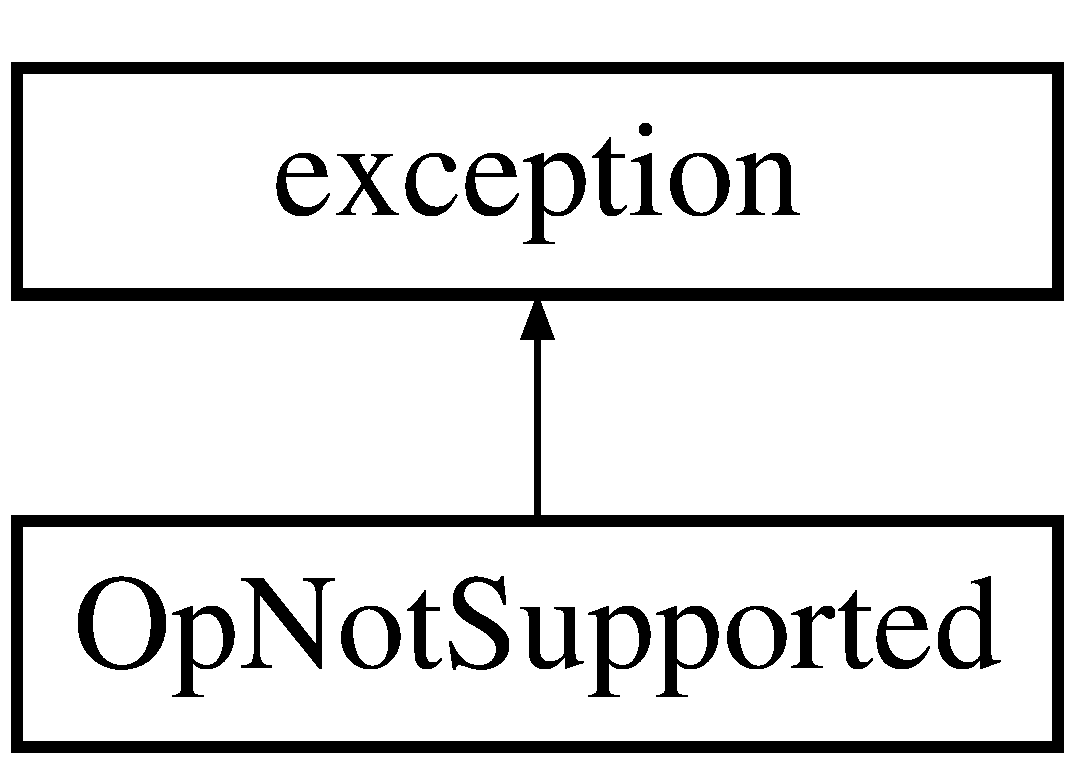
\includegraphics[height=2.000000cm]{class_op_not_supported}
\end{center}
\end{figure}
\subsection*{Public Member Functions}
\begin{DoxyCompactItemize}
\item 
\hypertarget{class_op_not_supported_ae538c9ab4dfbb4f82db960de61cb7458}{{\bfseries Op\+Not\+Supported} (std\+::string message)}\label{class_op_not_supported_ae538c9ab4dfbb4f82db960de61cb7458}

\item 
\hypertarget{class_op_not_supported_a2fea1b12d8fee8e97ee2c428cd62d7e0}{virtual const char $\ast$ {\bfseries what} () const   throw ()}\label{class_op_not_supported_a2fea1b12d8fee8e97ee2c428cd62d7e0}

\end{DoxyCompactItemize}


\subsection{Detailed Description}
Operation not supported/implemented. 

The documentation for this class was generated from the following files\+:\begin{DoxyCompactItemize}
\item 
M\+M\+K\+P\+\_\+\+Meta\+Heuristic.\+h\item 
M\+M\+K\+P\+\_\+\+Meta\+Heuristic.\+cpp\end{DoxyCompactItemize}

\hypertarget{class_or_lib___read}{\section{Or\+Lib\+\_\+\+Read Class Reference}
\label{class_or_lib___read}\index{Or\+Lib\+\_\+\+Read@{Or\+Lib\+\_\+\+Read}}
}


\hyperlink{class_or_lib___read}{Or\+Lib\+\_\+\+Read} Function Object reads from or\+Lib\+\_\+data and converts to common format \hyperlink{class_m_m_k_p_data_set}{M\+M\+K\+P\+Data\+Set}.  




{\ttfamily \#include $<$M\+M\+K\+P\+Data\+Set.\+h$>$}

\subsection*{Public Member Functions}
\begin{DoxyCompactItemize}
\item 
\hypertarget{class_or_lib___read_a74e1d387988c29eea5de937d8a02b576}{\hyperlink{class_m_m_k_p_data_set}{M\+M\+K\+P\+Data\+Set} \hyperlink{class_or_lib___read_a74e1d387988c29eea5de937d8a02b576}{operator()} (std\+::ifstream \&file)}\label{class_or_lib___read_a74e1d387988c29eea5de937d8a02b576}

\begin{DoxyCompactList}\small\item\em Convert input file to \hyperlink{class_m_m_k_p_data_set}{M\+M\+K\+P\+Data\+Set}. \end{DoxyCompactList}\end{DoxyCompactItemize}


\subsection{Detailed Description}
\hyperlink{class_or_lib___read}{Or\+Lib\+\_\+\+Read} Function Object reads from or\+Lib\+\_\+data and converts to common format \hyperlink{class_m_m_k_p_data_set}{M\+M\+K\+P\+Data\+Set}. 

Data can be found at \href{ftp://cermsem.univ-paris1.fr/pub/CERMSEM/hifi/MMKP/}{\tt ftp\+://cermsem.\+univ-\/paris1.\+fr/pub/\+C\+E\+R\+M\+S\+E\+M/hifi/\+M\+M\+K\+P/} . 

The documentation for this class was generated from the following files\+:\begin{DoxyCompactItemize}
\item 
M\+M\+K\+P\+Data\+Set.\+h\item 
M\+M\+K\+P\+Data\+Set.\+cpp\end{DoxyCompactItemize}

\hypertarget{class_population_generator}{\section{Population\+Generator Class Reference}
\label{class_population_generator}\index{Population\+Generator@{Population\+Generator}}
}
Inheritance diagram for Population\+Generator\+:\begin{figure}[H]
\begin{center}
\leavevmode
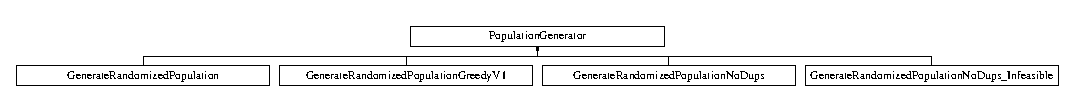
\includegraphics[height=0.918033cm]{class_population_generator}
\end{center}
\end{figure}
\subsection*{Public Member Functions}
\begin{DoxyCompactItemize}
\item 
\hypertarget{class_population_generator_a640e926b542c704b1f0ce1da143c81d8}{virtual std\+::vector$<$ \hyperlink{class_m_m_k_p_solution}{M\+M\+K\+P\+Solution} $>$ {\bfseries operator()} (\hyperlink{class_m_m_k_p_data_set}{M\+M\+K\+P\+Data\+Set} data\+Set, int population\+Size)=0}\label{class_population_generator_a640e926b542c704b1f0ce1da143c81d8}

\item 
\hypertarget{class_population_generator_a06498ef715cfb92f261e8f39a2c7da92}{bool {\bfseries not\+Included} (\hyperlink{class_m_m_k_p_solution}{M\+M\+K\+P\+Solution} solution, std\+::vector$<$ \hyperlink{class_m_m_k_p_solution}{M\+M\+K\+P\+Solution} $>$ population)}\label{class_population_generator_a06498ef715cfb92f261e8f39a2c7da92}

\end{DoxyCompactItemize}


The documentation for this class was generated from the following files\+:\begin{DoxyCompactItemize}
\item 
M\+M\+K\+P\+Population\+Generators.\+h\item 
M\+M\+K\+P\+Population\+Generators.\+cpp\end{DoxyCompactItemize}

\hypertarget{struct_t_l_b_o__parameters}{\section{T\+L\+B\+O\+\_\+parameters Struct Reference}
\label{struct_t_l_b_o__parameters}\index{T\+L\+B\+O\+\_\+parameters@{T\+L\+B\+O\+\_\+parameters}}
}


Parameters for customizing the T\+L\+B\+O algorithm.  




{\ttfamily \#include $<$M\+M\+K\+P\+\_\+\+T\+L\+B\+O.\+h$>$}

\subsection*{Public Attributes}
\begin{DoxyCompactItemize}
\item 
\hypertarget{struct_t_l_b_o__parameters_a85bb3efd9c225a720c243502388800a4}{int {\bfseries population\+Size}}\label{struct_t_l_b_o__parameters_a85bb3efd9c225a720c243502388800a4}

\item 
\hypertarget{struct_t_l_b_o__parameters_a2e65a62e1f51bbc5a5129cce67eb3c42}{int {\bfseries number\+Of\+Generations}}\label{struct_t_l_b_o__parameters_a2e65a62e1f51bbc5a5129cce67eb3c42}

\item 
\hypertarget{struct_t_l_b_o__parameters_a13cf7c6d4bd63924455180f2fc5708c3}{int {\bfseries generations\+Of\+N\+O\+P}}\label{struct_t_l_b_o__parameters_a13cf7c6d4bd63924455180f2fc5708c3}

\item 
\hypertarget{struct_t_l_b_o__parameters_a8dec005b886d2fc21eee7058d13005b5}{int {\bfseries classroom\+Size}}\label{struct_t_l_b_o__parameters_a8dec005b886d2fc21eee7058d13005b5}

\item 
\hypertarget{struct_t_l_b_o__parameters_a62d47e766b5a0431fbdcabcee7816751}{int {\bfseries multiple\+Choice\+Feasibility\+Mod}}\label{struct_t_l_b_o__parameters_a62d47e766b5a0431fbdcabcee7816751}

\item 
\hypertarget{struct_t_l_b_o__parameters_a602bb8be8c4f17ec7d70af33c9be36be}{int {\bfseries multiple\+Dim\+Feasibility\+Mod}}\label{struct_t_l_b_o__parameters_a602bb8be8c4f17ec7d70af33c9be36be}

\item 
\hypertarget{struct_t_l_b_o__parameters_ab4dead72475e9a945b2bed9358152e25}{bool {\bfseries add\+Random\+Teacher}}\label{struct_t_l_b_o__parameters_ab4dead72475e9a945b2bed9358152e25}

\item 
\hypertarget{struct_t_l_b_o__parameters_ac4a740ceafcea10ba072738868e4d297}{bool {\bfseries add\+Sim\+Annealing}}\label{struct_t_l_b_o__parameters_ac4a740ceafcea10ba072738868e4d297}

\end{DoxyCompactItemize}


\subsection{Detailed Description}
Parameters for customizing the T\+L\+B\+O algorithm. 

The documentation for this struct was generated from the following file\+:\begin{DoxyCompactItemize}
\item 
M\+M\+K\+P\+\_\+\+T\+L\+B\+O.\+h\end{DoxyCompactItemize}

\hypertarget{struct_t_l_b_o__statistics}{\section{T\+L\+B\+O\+\_\+statistics Struct Reference}
\label{struct_t_l_b_o__statistics}\index{T\+L\+B\+O\+\_\+statistics@{T\+L\+B\+O\+\_\+statistics}}
}
\subsection*{Public Attributes}
\begin{DoxyCompactItemize}
\item 
\hypertarget{struct_t_l_b_o__statistics_ac9b054ef9b104dd79be490cce135eb70}{int {\bfseries total\+Mutations}}\label{struct_t_l_b_o__statistics_ac9b054ef9b104dd79be490cce135eb70}

\item 
\hypertarget{struct_t_l_b_o__statistics_adf222336eb684d4182b10912d6459414}{int {\bfseries accepted\+Mutations}}\label{struct_t_l_b_o__statistics_adf222336eb684d4182b10912d6459414}

\item 
\hypertarget{struct_t_l_b_o__statistics_a6d0784f4a388c182068a831df5d0a246}{int {\bfseries total\+Infeasible\+Mutations}}\label{struct_t_l_b_o__statistics_a6d0784f4a388c182068a831df5d0a246}

\item 
\hypertarget{struct_t_l_b_o__statistics_aac5abfe2e303c6706b540e44d6b63528}{int {\bfseries made\+Feasible\+Mutations}}\label{struct_t_l_b_o__statistics_aac5abfe2e303c6706b540e44d6b63528}

\item 
\hypertarget{struct_t_l_b_o__statistics_afe6dc3034db769ef19814ca505bb7f77}{std\+::vector$<$ \hyperlink{class_m_m_k_p_solution}{M\+M\+K\+P\+Solution} $>$ {\bfseries unique\+Solutions}}\label{struct_t_l_b_o__statistics_afe6dc3034db769ef19814ca505bb7f77}

\end{DoxyCompactItemize}


The documentation for this struct was generated from the following file\+:\begin{DoxyCompactItemize}
\item 
M\+M\+K\+P\+\_\+\+T\+L\+B\+O.\+h\end{DoxyCompactItemize}

%--- End generated contents ---

% Index
\newpage
\phantomsection
\addcontentsline{toc}{chapter}{Index}
\printindex

\end{document}
